% Define document class. Important.
\documentclass[a4paper,twoside,openany]{report}

% Margener
%\setlength{\evensidemargin}{1cm}
%\setlength{\oddsidemargin}{1cm}

% Set up encoding. Latin1 since UTF-8 is fuckably difficult to work with.
% \usepackage[latin1]{inputenc}
\usepackage[latin1,utf8,ansinew]{inputenc}

% Variable, neat, references.
\usepackage{varioref}

% Load up bibliography.
\usepackage{natbib}
% Bibliography style.
\bibliographystyle{plain}

% Algorithm support.
\usepackage{algorithmic}
\usepackage{algorithm}
% Make algorithms appear as procedures instead.
\floatname{algorithm}{Procedure}
\renewcommand{\algorithmicrequire}{\textbf{Input:}}
\renewcommand{\algorithmicensure}{\textbf{Output:}}

% Image frames.
\setlength{\fboxsep}{0pt}
\setlength{\fboxrule}{0.5pt}

% Also, images.
\usepackage{graphicx}

% Todo notes here and there.
\usepackage[disable]{todonotes}

% Forbedrede floats.
\usepackage{float}

% Special symbols availability.
\usepackage{amssymb}

% CODE %
\usepackage{listings}
\usepackage{color}
\definecolor{gray}{rgb}{0.4,0.4,0.4}
\definecolor{darkblue}{rgb}{0.0,0.0,0.6}
\definecolor{cyan}{rgb}{0.0,0.6,0.6}
\lstset{
  basicstyle=\ttfamily,
  columns=fullflexible,
  showstringspaces=false,
  commentstyle=\color{gray}\upshape,
  basicstyle=\small,
  numberstyle=\footnotesize,
  numbers=left,
  captionpos=b,
  stepnumber=1,
  numbersep=10pt,
  tabsize=2,
  breaklines=true,
}
% Define markup of XML
\lstdefinelanguage{XML}
{
  morestring=[b]",
  morestring=[s]{>}{<},
  morecomment=[s]{<?}{?>},
  identifierstyle=\color{darkblue},
  keywordstyle=\color{cyan},
  morekeywords={id, target, type, category, value, point, correct, rows, width, time}% list your attributes here
}
% Define markup of C#
\lstdefinelanguage{CSharp}[Visual]{C++}
{
	identifierstyle=\color{darkblue},
	commentstyle=\color{green!70!black}\itshape ,
	stringstyle=\color{gray},
	sensitive=true,
	morestring=[b]",
	morestring=[b]',
	morecomment=[l]//,
	morecomment=[n]{/*}{*/}
}

% Neat-o referencer...o.
\usepackage{hyperref}
\usepackage{nameref}

% hack fra nettet.
% http://tex.stackexchange.com/questions/1230/reference-name-of-description-list-item-in-latex
\makeatletter
\let\orgdescriptionlabel\descriptionlabel
\renewcommand*{\descriptionlabel}[1]{%
  \let\orglabel\label
  \let\label\@gobble
  \phantomsection
  \edef\@currentlabel{#1}%
  %\edef\@currentlabelname{#1}%
%  \let\label\orglabel
  \orgdescriptionlabel{#1}%
}
\makeatother
% Rettehak. Meget lettere end \checkmark
\newcommand{\yes}{\checkmark}

% Let's put in a lot of niceness in the display, yeh?
\usepackage{fancyhdr} % Get some niceness into our headers.
\pagenumbering{arabic} % Ensure page numbering in our desired form.
\pagestyle{fancy}
% Page design from fancyhdr.
\fancyhead{}
\fancyfoot{}
\fancyhead[RO,LE]{\leftmark\\\rightmark}
\fancyfoot[C]{\thepage}
\setlength{\headheight}{23pt}
% Rewrite header and footer commands.
\renewcommand{\headrulewidth}{1.0pt}
\renewcommand{\footrulewidth}{1.0pt}

% Create a new command, HRule, to insert some nice horisontal rules on the title page.
\newcommand{\HRule}{\rule{\linewidth}{0.3mm}}

% New command for two figures, side by side.
\newcommand{\twofigs}[6]
{
	\begin{figure}[H]
		\begin{minipage}[b]{0.5\columnwidth}
		\centering\fbox{\includegraphics[width=0.8\columnwidth]{img/#1}}\caption{#2\label{#3}}
		\end{minipage}
		\hspace{0.5cm}
		\begin{minipage}[b]{0.5\columnwidth}
		\centering\fbox{\includegraphics[width=0.8\columnwidth]{img/#4}}\caption{#5\label{#6}}
		\end{minipage}	\end{figure}
}

% Sørg for at paragrafplads ikke spildes.
\raggedbottom

\begin{document}

\thispagestyle{empty}
\begin{center}
	%\includegraphics[width=15cm]{forside.png}\\~\\
	\hrulefill\newline
	\\
	\begin{LARGE}	
	\textbf{GIRAF Admin}
	\end{LARGE}
	\\
	\begin{large} 
	\textbf{An administrative addition to the GIRAF framework}
	\end{large}\\
	\hrulefill\newline
	%\hrule
	\\~\\
	Aalborg University, Second year in Engineering, Science and Medicine\\
	SW3, fall semester 2011	\\
	Project group SW305E11\\
\end{center}
\newpage
\thispagestyle{empty}
\mbox{}
\clearpage

\thispagestyle{empty}
\begin{titlepage}
\begin{nopagebreak}
\setcounter{page}{3}
{\samepage 
\begin{tabular}{r}
\parbox{\textwidth}{  \raisebox{11mm}{
\includegraphics[height=1.2cm]{img/aau-logo.pdf}}
\hfill \parbox{4.9cm}{\begin{tabular}{l}
{\sf\small \textbf{Det Teknisk-Naturvidenskabelige Basis{\aa}r }}\\
{\sf\small  \textbf{Software}} \\
{\sf\small Strandvejen 12-14} \\
{\sf\small Telefon 96 35 97 31} \\
{\sf\small Fax 98 13 63 93} \\
{\sf\small http://tnb.aau.dk}
\end{tabular}}}
\\
\end{tabular}

\begin{tabular}{cc}
\parbox{6cm}{
\begin{description}

\item {\bf Title:} 

XAT
  
\item {\bf Subject:} 

Screening

\end{description}

\parbox{8cm}{

\begin{description}
\item {\bf Project period:}\\
   P2, spring semester 2011\\
  \hspace{4cm}
\item {\bf Project group:}\\
  SW2B140\\
  \hspace{4cm}
\item {\bf Attendees:}\\
Jesper Riemer Andersen \\
Nicklas Andersen \\
Johannes Lindhart Borresen \\
Sam Sepstrup Olesen \\
Simon Reedtz Olesen \\
Kris Riisager \\
Jacob Karstensen Wortmann \\
  \hspace{2cm}
\item {\bf Supervisor:}\\
Karsten Jahn \\
\end{description}
}
\begin{description}
\item {\bf Edition:} 1.0
\item {\bf Number of pages:} \pageref{lastpage}
\item {\bf Appendix pages:} 12
\item {\bf Finished:} 24/5/2011
\end{description}
\vfill } &
\parbox{7cm}{
  \vspace{.15cm}
  \hfill 
  \begin{tabular}{l}
  {\bf Synopsis:}\bigskip \\
  \fbox{
    \parbox{6.5cm}{\bigskip
     {\vfill{\small The initializing problem of this rapport was to make an PC-administrations tool that would be able to administer Giraf system on a mobile device, that was made in a bachelor multi-project in 2011. But after interviewing the kindergarten teacher Kristine Niss-Henriksen from Birken the rapport focus on making a  digitized version of the children's contact book that simplify the communication between the kindergarten teachers and parents. 
This rapport describes the development of Giraf administration system with main focus on the contact book. This rapport includes the usage of models, prototypes, the klient-server architecture, and the implementation of the model-view-controller design. Furthermore to evalutate the system both unit testing and usability testing used. 
     \bigskip}}
     }}
   \end{tabular}}
\end{tabular}}
\\ \\
\noindent{\footnotesize\emph{The content of this rapport can be used freely; however publication (with source material) may only occur in agreement with
the authors.}}
\end{nopagebreak}
\end{titlepage}
\newpage
\thispagestyle{empty}
\mbox{}

\chapter*{Preface}
The following report has been made as a part of the SW3 project for the second-year students of software engineering at Aalborg University. The report is based upon the project proposals given to the students at the beginning of the semester and written in parallel with the lectures \emph{Algorithms and Data Structures}, \emph{Systems Development and Design}, \emph{Implementation and Evaluation of User Interfaces}. Source material can be found in the last part of the report.

The group would like to thank the Kindergarten Birken and their kindergarten teacher Kristine Niss-Henriksen for her participation in this project. This report and product is an expansion of the multi-project from spring 2011 made by the groups: s601a, s601b, s601c and s601e, and we want to thank these groups for the pre-work. Finally, we want to thank our supervisor Ulrik Nyman, for his continued envolvment and support during this process.

\phantom{Luft}

\phantom{Luft}

\begin{table}[H]
	\centering
		\begin{tabular}{c c c}
			\underline{\phantom{JAERJAERJAERJAER}} & \underline{\phantom{JAERJAERJAERJAER}} & \underline{\phantom{JAERJAERJAERJAER}} \\
			Birgir M. Eliasson			& Christoffer Kjeldgaard       	& Johannes L. Borresen 			\\
			&&\\
			&&\\\\\\
			\underline{\phantom{JAERJAERJAERJAER}} & \underline{\phantom{JAERJAERJAERJAER}} & \underline{\phantom{JAERJAERJAERJAER}} \\
			Lisbeth	Nielsen			& Ren� K. H. Andersen 					& Toke N. Olsen				\\									
		\end{tabular}
\end{table}

\newpage
\thispagestyle{empty}
\mbox{}

%\newpage
%\thispagestyle{empty}
%\mbox{}

%\newpage
%\thispagestyle{empty}
%\mbox{}
%\fancyhead{}
%\fancyfoot{}
%\fancyhead[RO,LE]{\leftmark\\\rightmark}
%\fancyfoot[C]{\thepage}
%\setlength{\headheight}{23pt}

% Fjern headeren for indholdsfortegnelsen.
%\fancyhead{}
%\fancyfoot{}
%\fancyhead[RO,LE]{\leftmark}
%\fancyfoot[C]{\thepage}
%\setlength{\headheight}{23pt}% Indholdsfortegnelser etc.
% Dybde for visning af niveauer.
% Dybde af niveaut�lling generelt.
\setcounter{secnumdepth}{3}
\setcounter{tocdepth}{1}

\tableofcontents

% Introduktion
\chapter{Introduction}

The purpose of this project is to create a user-friendly web-application that makes the user able to create entries in an web-based contact book which should replace the current china book version and make it easier for the kindergarten teachers and guardians to communicate with each other. Furthermore, this project will try to establish a foundation, such that the functionalities created in this project can be added to the current GIRAF system. 

The project is created as addendum to other GIRAF projects, casting light on how these additions can be made to the already implemented software, moreover how it would improve the working environment for kindergarten teachers working with autistic children. 
Specifically, one institution contributed throughout the project, Birken, which is a kindergarten for children with a need for special care and a alternative learning environment. Birken is situated in Vodskov in the Northern Denmark region.

The primary contact from Birken, Kristine Niss-Henriksen, has been included in this project because of her knowledge about children with autism and experience with today's technology. Furthermore, she contributed with design ideas for the front-end of the software and in testing and providing feedback on prototypes, which helped us in creating the final product.

The project was originally based on creating an administration tool for the GIRAF tablets, making it possible to manage and push application settings to registered devices. However, from the interviews made with Kristine we learned that this functionality was not a pressing issue; adding the aforementioned contact book functionality had a higher priority.  

Some words are defined in the list below for the reader's convenience
\begin{itemize}
\item{Guardians = Parents, or persons which has custody over the child}
\item{Kindergarten teacher = In this context, a person working with autistic children}
\item{The GIRAF system is the result of a multi-project made in spring 2011 which is a android based operating system for a mobile device that creates a safe environment for children with disabilities.}
\end{itemize}
\section{Autism}
Autism is defined as a developmental disorder, which effects the brain's ability to develop communication- and social skills. Autism often appears during the first three years of a child's life, and the disorder is often diagnosed during the following years.
The definition of autism is broad, which means that some autistic children have different symptoms than their peers, but to diagnose, the \textit{Autism Spectrum Disorder} which consists of three basic symptoms, is used. These three symptoms are listed below.
\begin{itemize}

  \item{Lack of communications skills.}
   \begin{itemize}
     \item{The child has slow or no development of language. The child may use gestures to communicate instead of words, it may have trouble with maintaining focus in a conversation or have trouble starting a conversation.}
   \end{itemize}
   
  \item{Lack of social skills.}
   \begin{itemize}
     \item{The child may have difficulty making friends. The child may be withdrawn or may not respond to eyecontact and smiles. The child may treat other children and/or adults as objects. The child may rather play alone than play with others.}
   \end{itemize}

  \item{Repetitive and/or compulsive behavior}
    \begin{itemize}
      \item{The child may have unusual distress if particular routines are changed or not being followed. The child may perform repeated body movements. \cite{autism}}
    \end{itemize}
  
\end{itemize}

The exact causes of autism are still unknown, but are supposedly a combination of different factors. Some possible causes, which have been suspected though not proven, are listed below:

\begin{itemize}
  
  \item{Diet}
  \item{Changes of the digestive tract}
  \item{Poison by mercury}
  \item{The body's lack of ability to utilize vitamins and minerals properly}
  \item{Sensitivity against vaccines\cite{autism}}
  
\end{itemize}

Even though the factors listed above are mostly physical, the autism disorder is supposedly linked to unusual biology and the chemistry of the brain.
It seems that genetics are an important factor. E.g. it is more likely for identical twins, than fraternal twins or siblings, to both be autistic\cite{autism}.
\section{Communication with an autistic child}
The parents and kindergarten teachers use Picture Exchange Communication System or \emph{PECS}, to communicate with an autistic child and this system has been successfully used for over 10 years in the USA\cite{centerAutism}. The communication tool consists of pictures or pictograms that represent something the child should do or wants to do. This can be a drawing of an apple, signaling the child which fruit to eat. 

This form of communication is used in kindergartens for children with special needs e.g. children with autism. Mostly these pictograms are printed from a computer program called \emph{Boardmaker}, which has many different pictograms that can be edited to make it easier for the child to understand\cite{centerAutism}. This could be when the child needs to put on a blue t-shirt, then the adult gives the child a pictogram of a blue t-shirt and the child understands. It can be confusing for the child if the actual t-shirt is one color and the one on the pictogram is another.

The PECS can also be used as a schedule for the children. In the kindergarten Birken pictograms are used as a daily schedule, where kindergarten teachers put the pictograms along a column on the wall and each row represents a single activity.
The child is taught to take the pictogram of the finished activity and put it away in a box. Later, the pictogram can be put on next day's schedule, without confusing the child about whether the activity is finished or not.
%Later in the child's development the pictogram would be put next to the schedule, but the child would still understand that this activity is finished.


% 1. analyse
\part{Analysis}


\chapter{Problem analysis}

In this chapter we take a look at the reports from previous giraf-developing groups. By collecting information from them, we can better understand the initial problem and better analyse the current problem.

\section{The multi-project GIRAF}
Our project is based upon the bachelor multi-project from spring 2011, in which four groups developed the GIRAF system for mobile devices running \textit{Android}. The concept of the GIRAF system is to make an \textit{Android} based software system, which has the purpose of helping autistic children, their parents and kindergarten teachers. The idea is to give every child a mobile device for everyday use. The parents and/or kindergarten teachers can then administrate the applications within the GIRAF system. Furthermore the system should make it easier for the child to communicate with the parents or kindergarten teachers. 

\subsection{FACTORS for the multi-project Giraf system}
The FACTORS criteria are used to support the preparation of a system definition. In the following, the FACTORS for the multi-project GIRAF will be covered\cite{giraffactors}. The definition of each criterion is based on OOA \& D\cite{OOAD}.

\subsubsection{Functionality} 
Describes the systems functions that support the application domain tasks. That is, defining
what the system is able to do.
\begin{itemize}
	\item The system should offer installation of new applications and make it possible to administrate common settings by need. 
	\item The system should mask the normal functionalities of the unit to the user.
	\item Furthermore, the system should give the opportunity to control the usage of and access to system and user profile settings as well as applications according to the current time, and location of the unit.
	\item The system should be delivered with a number of pre-installed applications which are customizable for the user.
	\item The system should have a framework with objects like a calendar, ready for development of GIRAF compliant software.
\end{itemize}

\subsubsection{Application Domain} 
Concerns those parts of an organization which administrate, monitor, or control a
problem domain.
\begin{itemize}
	\item Children with limited mental capabilities due to handicap or age, making it hard for them to handle the complexity of a normal smart-phone or tablet OS. 
	\item Parents and kindergarten teachers will be in charge of administrating the system.
\end{itemize}

\subsubsection{Conditions} 
Covers conditions under which the system will be developed and used.
\begin{itemize}
	\item The system should be simple and intuitive to use. 
	\item The system should be developed so that it is customizable to the individual child and it's disabilities.
	\item Furthermore, it should allow parents to limit the functionality of the system. 
	\item To allow other application developers to continue to develop the system and further applications, the system should be maintainable.
\end{itemize}

\subsubsection{Technology} 
Covers the technology used to develop the system and the technology on which the system will
run.
\begin{itemize}
	\item The system must run on \textit{Android} touch devices such as smart-phones and tablets. Different hardware should be supported, although it is required that the units are running \textit{Android} 2.2 or newer. 
	\item The system should mainly be developed using Java and the \textit{Android} SDK version 8 for \textit{Android} 2.2.
\end{itemize}

\subsubsection{Objects} 
Describes the main objects in the problem domain.
\begin{itemize}
	\item A smart-phone or tablet device. 
	\item The \textit{Android} platform. 
	\item Global system- and application specific settings. 
	\item Applications.
	\item Administrative application for a stationary device.
\end{itemize}

\subsubsection{Responsibility} 
Covers the systems overall responsibility in relation to its context. That is, how the system would interact with the tasks to be solved using the system.
\begin{itemize}
	\item The system should act as an assistive tool by providing pre-installed applications developed to aid and entertain the small-aged and disabled children using the system. 
	\item Furthermore, the system should provide the opportunity to install other third party applications. 
	\item Through a home menu, the system should in accordance with the location, the user profile as well as the global settings of the system control which applications the user is allowed to access.
\end{itemize}

\subsection{Multiproject system definition}

\textit{"A simple and intuitive module based single user system for Android touch devices, such as smart-phones and tablets. By masking the normal interface of an Android device, the device should offer functionality that is suitable for the intended user.
The system should be responsible for aiding and entertaining children with limited mental capabilities due to mental handicap and/or age, having a difficult time handling the complexity of a normal smart-phone or tablet OS. Guardians should be able to administrate the system by controlling selected application-, system and user-specific settings through an administration interface on a stationary device. Based on these settings, as well as the location of the unit, a home menu should be responsible for providing access to applications that conforms to the current settings and the state of the system. It should be possible for any third party to develop and provide additional applications to the system. Beyond that, the system must be delivered with a set of pre-installed applications consisting of a visual, day-to-day, planning tool, and a PECS application. The system should be developed using Java and the recent version of the Android SDK. It is expected that the system supports Android 2.2. Furthermore, it is expected that the system is maintainable to such a degree, that it allows other developers to keep developing the system as well as applications to the system after this semester."} citation from the system definition in the Administration Module for GIRAF.\cite{giraffactors}

\subsection{The project result}
From researching previous groups' reports, the problem being addressed seems to be the autistic child's need for structure in every-day life and to do that, they digitized some tools. These tools are listed below.
\begin{itemize}
	\item a picture communication program called DigiPECS
	\item a visual schedule called aSchedule
\end{itemize}

To run all this on a mobile device, a launcher was developed specifically for the GIRAF system and a simple interface that masks the underlying \textit{Android} system. A specific marketplace for GIRAF apps was designed and partially implemented, where GIRAF users could update already installed apps or install new apps. The launcher also makes an administrator environment available to the parent or kindergarten teacher where they can install apps, edit settings and generally administer the device.
The tools that were digitized have been around in other forms for some time now, where they already simplify and make daily-life structure easier as well as help children, that are slow to develop, with communication.

The group who worked on the administrator environment concluded that an administration interface, for a stationary device would be nice to have, which is the background for this project.
Our focus is therefore not so much on the children but on the kindergarten teachers and the parents of the children. Where the administration interface should help the parents and kindergarten teachers to administer and manage the mobile devices using the GIRAF-administration system.\cite{giraffactors}

\section{Illustration of the system}
The reason for making a rich picture is to help one understand the interaction within a specific technology and/or product\cite{OOAD}. The drawing in Figure \vref{fig:Rig billede} is an overview of how the users (parents and kindergarten teachers) and the child would interact with the mobile device. Under the assumption that the multi-bachelor project \textit{GIRAF} has been implemented in everyday life, we want to show how it could be improved with an administrator program on the computer.

The mobile device is primarily used by the child as a communication tool by using using the application DigiPECS or aSchedule, but games can also installed to entertain the child. As a communication tool the child can ask for the user's help and the user can also use it to communicate with the child or tell the child to e.g. wash your hands before dinner. 
The users also need to use the mobile device when they want to add or edit something on the device e.g. schedule the next day's activities in aSchedule.  

 
The problem with the current \textit{GIRAF} system is that both the administrator and child need the same mobile device which could be at the same time. Some children will consider the mobile device theirs and therefore will not hand it over to the user or do so with much frustration. To resolve this problem without changing the mobile device primarily function, a computer program could be made, such that the user could administer the mobile device from a computer via some form of a wireless connection. This picture is shown in \vref{fig:Rig billede}. 

\begin{figure}[ht]
	\centering
		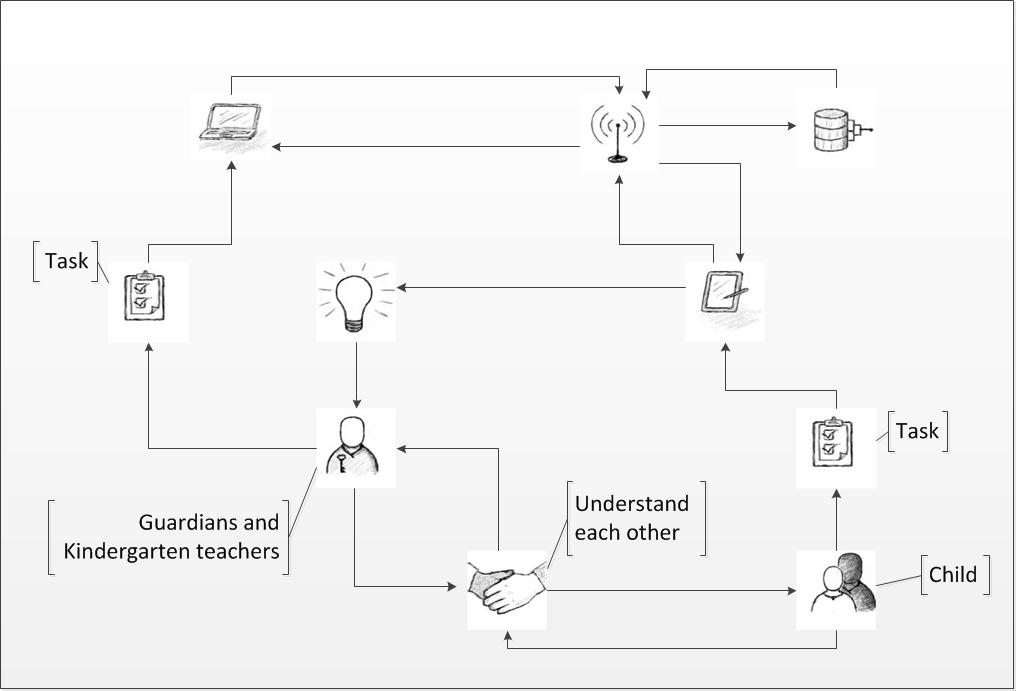
\includegraphics[width=1.00\textwidth]{img/Rig_billede2.jpg}
	\caption{The child uses the tablet to communicate with the parent or kindergarten teacher, such that the child and adult understand each other. The parent or kindergarten teacher uses a computer to administrate the tablet}
	\label{fig:Rig billede}
\end{figure}

In our project we want to make it possible to use a computer to change the mobile device setting, but our primary focus will be to make a digitized version of the contact book so that kindergarten teachers and parents, easily and quickly, can exchange information. The kindergarten teachers would then be able to write and send a summary of the child's activities including pictures of the involved activities to the parents. This is the base for our system definition.    
\section{Kindergarten Birken}
The kindergarten teacher is a very important person in the life of an autistic child. The kindergarten teacher is the person who helps and guards the autistic child. The kindergarten teacher and the child develop a special relationship to each other. The kindergarten teacher follows the child in a some of its everyday life and in the case of Birken, the kindergarten teachers follows each child individually in 17 hours each week. Employees from Birken have been included in the projected by the groups in the multi-project and in this project, we have had interviews with the kindergarten teacher Kristine Niss-Henriksen.


\subsection{PACT}
%ulriks kommentar:"Taler I om den nuv�rende situation eller om systemet her?" bliver allerede sagt her
After the first interview with Kristine, which is in appendix \vref{first_interview_birken}, we decided to include a digitized version of their contact book in our project. The contact book is primarily a communication tool that the kindergarten teachers and the parents use to write messages to each other concerning the child and this book is then transported with the child.  

A PACT analysis was made on the current use of the contact book based from the information gathered from the interview, see PACT model in Figure \vref{fig:PACT}. PACT is an acronym for People, Activities, Contexts and Technologies, and this analysis is general use for understanding how people undertake activities in a certain context often using some form of technology. The individual parameters are described in their respective headers in our PACT. 

\begin{figure}
	\centering
		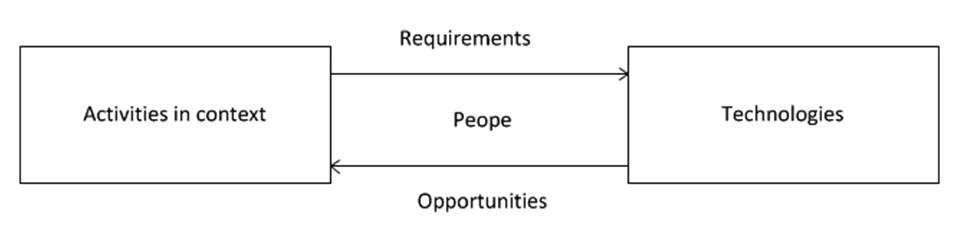
\includegraphics[width=0.70\textwidth]{img/PACT.png}
	\caption{PACT model}
	\label{fig:PACT}
\end{figure}



\subsubsection{People - the kindergarten teacher}
Kristine is in her thirties and is a fully educated pedagogue. Beyond this she has taken several degrees and courses focusing on the needs of children with mental handicaps, all resulting in her now working at Birken.

She takes care of a few selected children of those attached to the kindergarten, an activity that requires almost constant supervision while they are present. Kristine and her colleagues yearn for solutions that can ease and improve their daily work, particularly within the domains of communication with the children and their parents. Very notably, the time required to add a picture to an entry in the child's contact book is so severe that she cannot do it very often, a hindrance that bothers her. She would very much like to be able to attach an image to the book every day to improve the dialogue between child and parent.

\subsubsection{Activities}
\begin{itemize}
	\item Each day an entry is written in the contact book of every child, detailing the highlights of the day. It may be a single sentence or a paragraph with a picture of the child engaging in an activity. This is done by the kindergarten teachers, but entries may be commented on or entered a new by parents with any important thoughts.
	\item If a picture is to be added, first the picture is taken with a digital camera, imported into a desktop computer, then cropped, resized or rotated as necessary. Finally, the image is printed onto paper, cut out and glued into the contact book.
	\item Child and parent will sit down with the book, using the image in the book (if present) as a starting point for dialogue about the day, continuing through available pictograms.
\end{itemize}

\subsubsection{Contexts}
There are three contexts based on the three activities, two of them sufficiently similar to be written as one.
\begin{itemize}
	\item When compiling an entry in the contact book, the kindergarten teacher or guardian will sit by themselves, the child occupied either with their own devices or the supervision of someone else. 
	\item When discussing the entry in the book, however, child and parent are together.
\end{itemize}

\subsubsection{Technology}
Currently, two hardware technologies are in play: A digital camera, and a personal computer.
An image manipulation suite is used to edit the photographs. Possibly,  a Windows pre-installed application like MS Paint.

\subsubsection{Conclusion}
Even at a glance, several possible improvements can be suggested that make use of IT. Central are the notions of digitizing the contact book and easing the creation of images by using a mobile device with image manipulation software capable of the actions necessary.
\\
\\
\\
\subsection{Problem formulation}
In our project we want to make it possible to use a computer to change the mobile device settings, but our primary focus will be to make a digitized version of the contact book so that kindergarten teachers and parents, easily and quickly, can exchange information. The kindergarten teachers will then be able to write and send a summary of the child's activities including pictures of the involved activities to the parents. This is the base for our system definition.

\chapter{System definition}
In this chapter a FACTORS analysis and a system definition (that will list the demands for the digitized contact book), is outlined.

\section{FACTORS}
This is a FACTORS analysis of the contact book, a communication tool for parents and kindergarten teachers. The contact book should be available from the mobile device, so that a kindergarten teacher can snap a picture, write a post and upload it for the parent to read. FACTORS is a tool to define a product.

\subsection{Functions}
The contact book has a number of functions:
\begin{itemize}
	\item{Write a post of the day�s activites for the parents and kindergarten teachers to read.}
	\item{Both kindergarten teachers and parents should be able to edit and delete posts.}
	\item{Take, upload and edit pictures for the contact book. Furthermore it should be possible to attach a picture to the post of the day.}
	\item{The picture editor should include crop, resize and rotate.}
	\item{It should be possible to upload posts from both a mobile device and a PC.}
\end{itemize}

\subsection{Application domain}
The scope for the contact book concerns the kindergarten teachers and parents and to some degree the autistic children:
\begin{itemize}
	\item{The kindergarten teacher should have access to the contact book of each child in an associated group. They should be able to upload/edit pictures and add them to the contact book.}
	\item{A parent should only be able to read the contact book of their own child and be able upload/edit pictures.}
	\item{The child should have access to the contact book but without editing privileges.}
\end{itemize}

\subsection{Conditions}
There are several requirements for the contact book to work:
\begin{itemize}
	\item{There has to be synchronisation between mobile devices and the platform.}
	\item{It should be easily accessed by people with little IT-experience, as we have very little knowledge about the users, especially the parents.}
\end{itemize}

\subsection{Technology}
There are a couple of technological requirements for the contact book to work:
\begin{itemize}
	\item{The platform should be supported by both mobile devices as well as PC's.}
	\item{A database to store information, such as user credentials.}
  	\item{A specially designed framework to handle the contact book application.}
	\end{itemize}

\subsection{Objects}
The main objects related to the contact book:
\begin{itemize}
	\item{Mobile devices such as tablets or smartphones.}
	\item{The autistic children as they can read the contact book.}
	\item{Pictures taken for the contact book.}
	\item{The parents and kindergarten teachers as the contact book serves as a communication between the two.}
	\item{``A Day'', as the contact book is most likely edited from day to day and does not matter from i.e. week to week.}
\end{itemize}

\subsection{Responsibility} 
The main idea behind this contact book is to:
\begin{itemize}
	\item{Aid to the completion of writing and adding pictures to posts.}
	\item{Give an administrative tool to manage the contact book.}
	\item{Improve the communication between kindergarten teacher and parent aswell as the communication between a parent and it's child.}
\end{itemize}

\section{System definition}
The contact book software should primarily be a tool for enhancing communication between parents and kindergarten teachers, and secondly a helping tool for the child to better communicate with others. It should enable and store daily communication with text and pictures between the parents and kindergarten teachers. This should be implemented on a platform, supported by both mobile devices and PC's.
\newpage


% 2. Designing the product
\part{Designing the product}

\chapter{Modeling the product}
After analysing the problem and the solution provided by previous \emph{GIRAF} project groups, we can begin designing the product.
This modeling chapter contains a class diagrams of the GIRAF-W-11 framework, that would have to be designed and implemented before a fully functional contact book could be implemented. Furthermore, a function list for GIRAFAdmin.

\section{Modeling of GIRAF-W-11}
To understand how users, children and applications will be represented and connected in the system, a model has been made with only the most important classes included. This model is in figure \vref{fig:classOversigt}. The system we are developing, is called \emph{GIRAF-W-11} which then would have one user and many applications. As shown in the figure the \emph{User} would either be a \emph{Parent} or a \emph{Kindergarten teacher}. In the model the \emph{User} has a connection with a \emph{Child}, who also has a connection to its \emph{Mobile device}.

In reality it is possible for the child to have more than one device and that has been taken into account. This also means that there is an indirect connection between \emph{User} and \emph{Mobile device}, which has a \emph{GIRAF mobile application} installed. To administer a \emph{GIRAF mobile application} through \emph{GIRAF-W-11}, the corresponding \emph{GIRAF application administrator} must be used.

 However, those \emph{GIRAF administration applications} that do not exist for mobile devices, are considered a \emph{User application}. This is all represented in the model in figure \vref{fig:classOversigt}.


\begin{figure}[!ht]
	\centering
		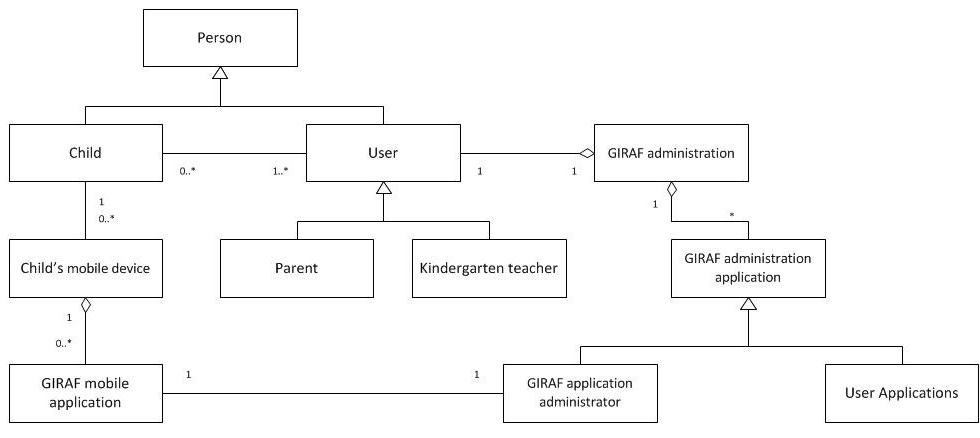
\includegraphics[width=1.00\textwidth]{img/classOversigt.jpg}
	\caption{The model of GIRAF-W-11}
	\label{fig:classOversigt}
\end{figure}
\newpage
\newpage
\section{UI functions}
In this section a list of functions, regarding the visual part of the system will be laid out. This is done to give a better understanding of which function that is needed of the GIRAF-W-11. The functions are grouped by an headline that should be a part of the GIRAF-W-11. However, not all function was implemented due to the limited time. 
  
\\
\\
Function types:
\begin{itemize}
\item{Update: Functions of this type are activated by an event in the problem area. Result: state-change in the model.}

\item{Signaling: Functions of this type are activated by state-change in the model, resulting in reaction in surroundings. Reaction can be a presentation for the users involved in the scope or direct intervention in the problem area.}

\item{Readings: Functions of this type are activated by the need of information in a user's tasks. Result: system displays relevant parts of the model.}

\item{Calculation: Functions of this type are activated by the need of information in a user's tasks, consisting of a calculation, which involves information from the user and the model. Result: Displaying the result of the calculation.}

\end{itemize}

The simple, medium, complex tags indicate how simple or complex the functions are to implement according to the development group.

\begin{table}[!ht]
\centering
\begin{tabular}{ l  c  c }

Login Screen: &  & \\ \hline
\textit{Function name} & \textit{Function complexity} & \textit{Function type} \\ \hline
login & Simple & Update \\ \hline
forgotPassword & Simple & Update \\ \hline
register & Medium & Update \\ \hline
\end{tabular}
\caption{Login screen functions}
\label{tbl:loginscreen}
\end{table}

\begin{table}[!ht]
\centering
\begin{tabular}{ l  c  c }

Newsfeed: & & \\ \hline
\textit{Function name} & \textit{Function complexity} & \textit{Function type} \\ \hline
getNews & Simple & Readings \\ \hline
addNewsPost & Medium & Update \\ \hline
canUserPost & Simple & Signaling \\ \hline

\end{tabular}
\caption{News functions}
\label{tbl:newsfeed}
\end{table}

\begin{table}[!ht]
\centering
\begin{tabular}{ l  c  c }

Main menu: & & \\ \hline
\textit{Function name} & \textit{Function complexity} & \textit{Function type} \\ \hline
signOut & Simple & Update \\ \hline
getMyAccount & Simple & Readings \\ \hline
getGroup & Medium & Update \\ \hline
getGroups & Medium & Readings \\ \hline
getChildList & Simple & Signaling \\ \hline
getAppList & Simple & Signaling \\ \hline
setView & Complex & Readings \\ \hline

\end{tabular}
\caption{Main menu functions}
\label{tbl:mainmenu}
\end{table}

\begin{table}[!ht]
\centering
\begin{tabular}{ l  c  c }

Contact book: & & \\ \hline
\textit{Function name} & \textit{Function complexity} & \textit{Function type} \\ \hline
getMessage & Medium & Readings \\ \hline
getMessageList & Medium & Readings \\ \hline
addNewMessage & Medium & Update \\ \hline
getCurrentUser & Simple & Readings \\ \hline
uploadImage & Medium & Update \\ \hline
addNewReply & Medium & Update \\ \hline

\end{tabular}
\caption{Contact book functions}
\label{tbl:contactbook}
\end{table}


\chapter{Prototyping}
\section*{Overview of process}
Different prototypes were used to decide, how the program should interact with the user and how the final user interface should be designed. In the following sections three different prototypes will be shown along with their work process and an explanation of related decision making.
The first prototypes were drawings on a blackboard or a piece of paper that were later converted to an HTML prototype \vref{program_tools_html_css}. In this process three group members designed the first prototype and presented it to the group. The group discussed points of improvements which led to a new design of the prototype. The HTML prototype was shown to kindergarten teacher Kristine Niss-Henriksen, in the second interview which is summarized in appendix \vref{sec_interview_birken}.

\section{The first prototypes}
After the first prototype was presented, each page was drawn on to a blackboard where the changes were more manageable. One of the first blackboard designs was the page ``Settings'', which contained information such as the child's name and abilities, shown in Figure \vref{fig:firstProto}. This is a primitive design with two menus, one horizontal and one vertical, the horizontal axis has all children and groups of children, the vertical axis has all the applications on a child's device, that the user can administer. This menu will be further explained in the section\vref{menus}. 

\begin{figure}[!ht]
	\centering
		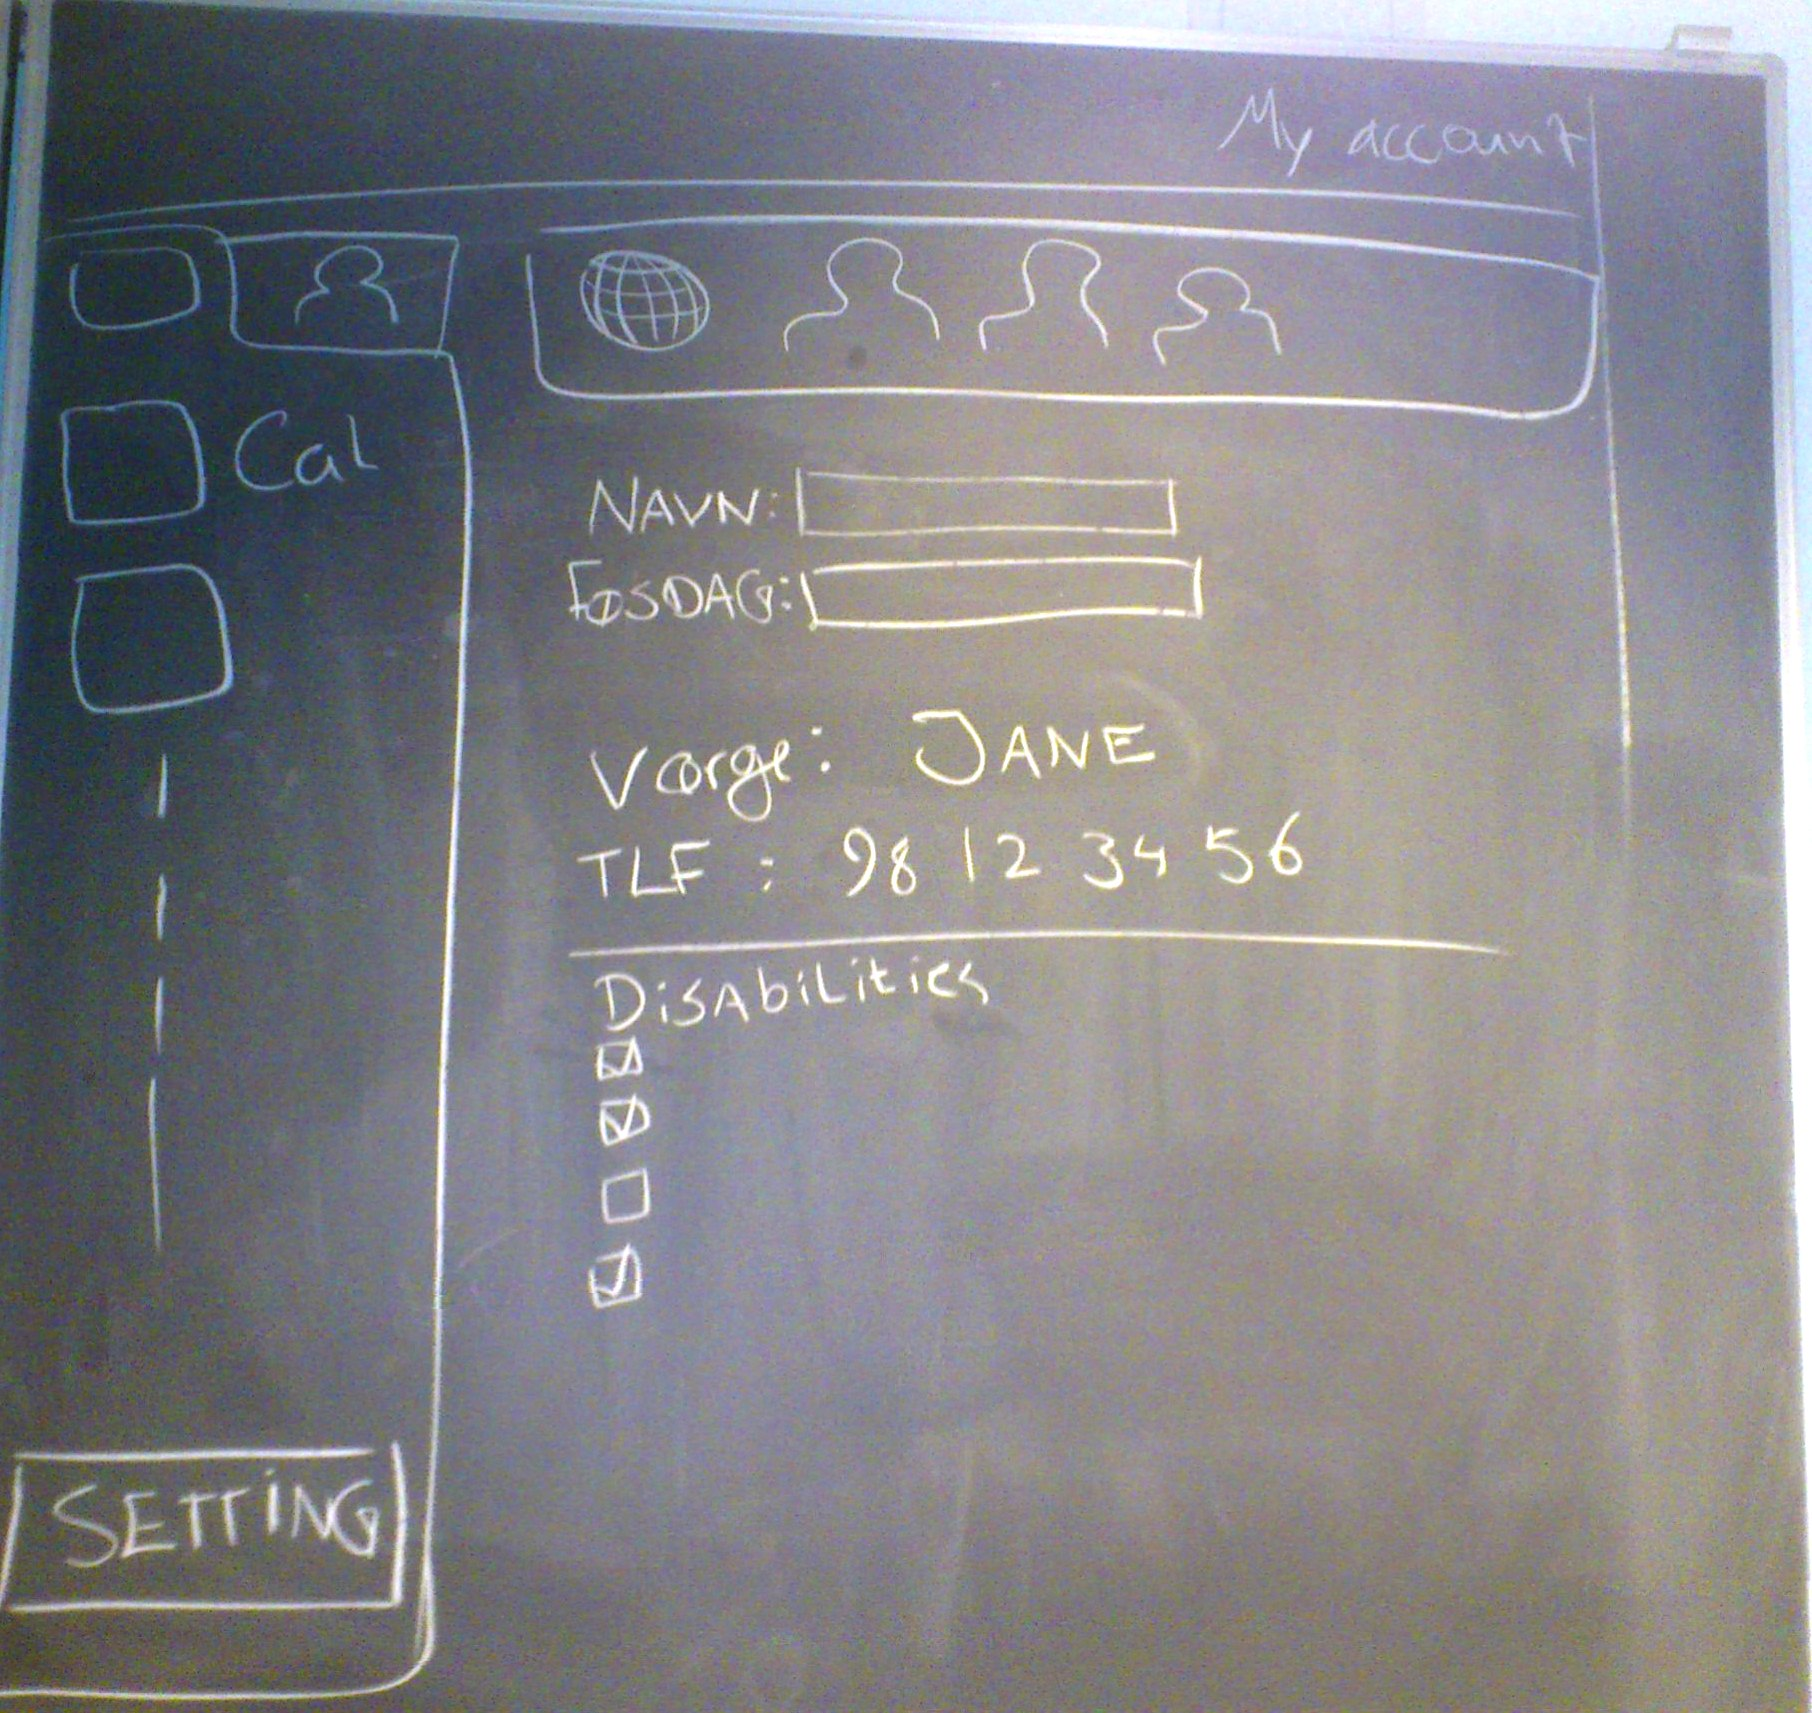
\includegraphics[width=0.60\textwidth]{img/firstproto.jpg}
	\caption{Black board design of the interface}
	\label{fig:firstProto}
\end{figure}


The group members disagreed on how to get into the ``Settings'' page in the first design. Reason being that the user would have to choose a child in the top horizontal menu and the press the ``Settings'' button in the vertical menu, which is located among GIRAF applications. Especially the location and the naming of the ``Settings'' button were discussed because the user could get the impression that they administer a child like an application and thereby creating confusion. To solve this it was suggested that this page should be in ``My Account'' instead; where the user would also be able to change their own personal information. The prototype design was not changed, and ``Settings'' page was never implemented.

\section{The HTML prototype}
For the second interview with Kristine Niss-Henriksen, an HTML prototype was made from the primitive prototypes. The Figure \vref{fig:contactbook} is two screen shoots from the child Jack's contact book where the right side of the figure is a light box with an entry from the contact book. The contact book is inspired by a calendar because, for each date, it can have entries which the user can click on. When clicked, a light box pops up that contains the message and pictures. If the user has not seen the message before, the signal ``Ny!'' in the right side should be visible. The user is able to fold and unfold the entries for each date, to see or hide the entries in the contact book. 

\begin{figure}[!ht]
	\centering
		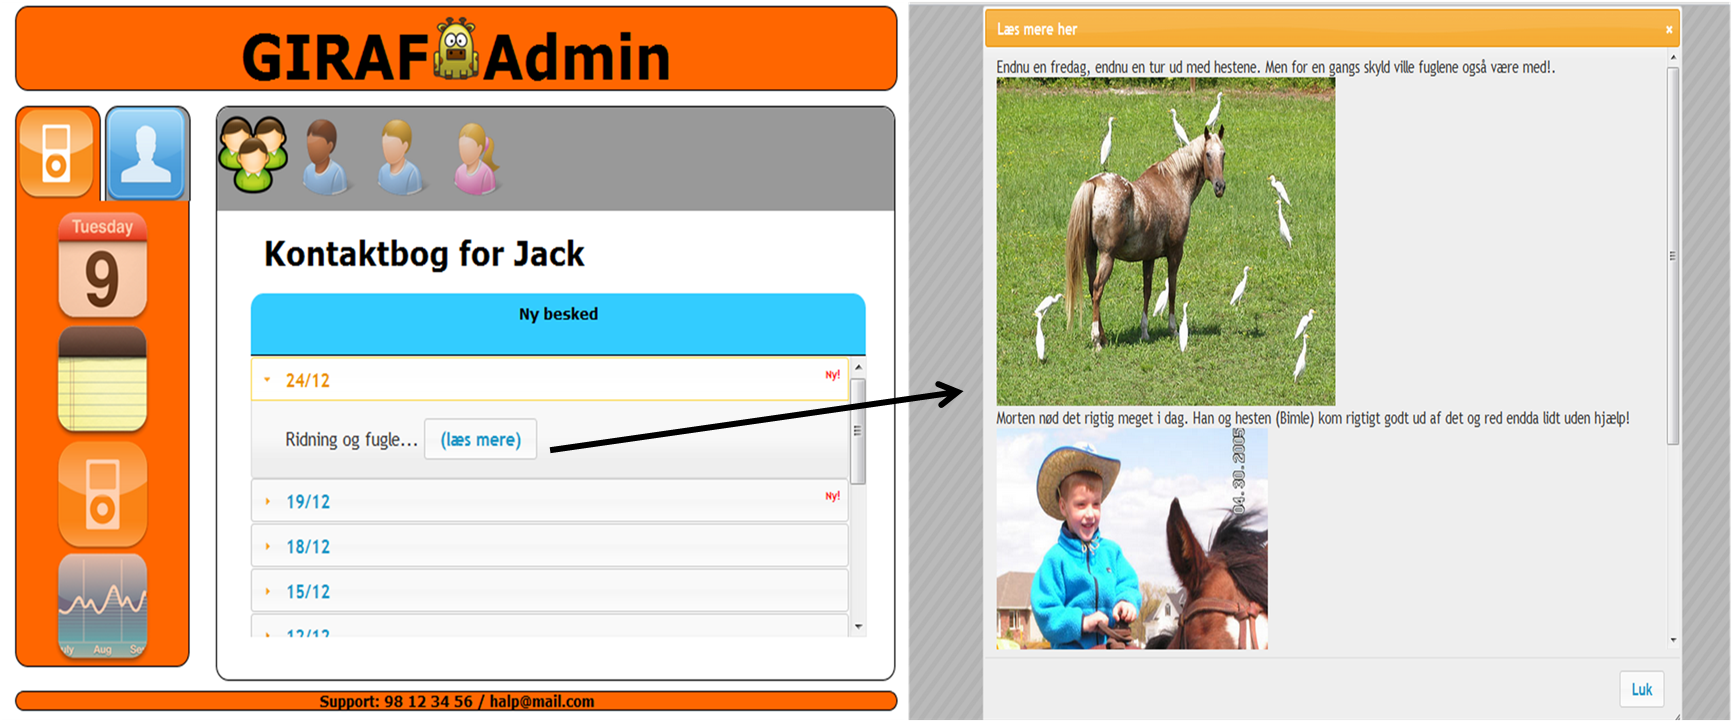
\includegraphics[width=1.00\textwidth]{img/contactbook.png}
	\caption{Prototype of the contact book and the light box with an entry}
	\label{fig:contactbook}
\end{figure}

\subsection{The menus}
\label{menus}
As it was pointed out earlier the GIRAF applications' administrators are represented on the vertical menu, as an icon that should identify the application administrator. The children's devices are represented on the horizontal menu where the single child's device is identified from a picture and the group is identified by an icon representing a group of children. However this representation can be mirrored such that the children's devices are represented on the vertical menu and the applications are represented on the horizontal menu, which is shown in Figure \vref{fig:menus}. The black circle indicates which of the menus is represented in the vertical menu. This menu was not implemented because it would take too much of the space on the screen, and it could also be a confusing navigation path for the user, without gaining any new functionality. In the next prototype this menu was replaced with two vertical menus side by side.

\begin{figure}[!ht]
	\centering
		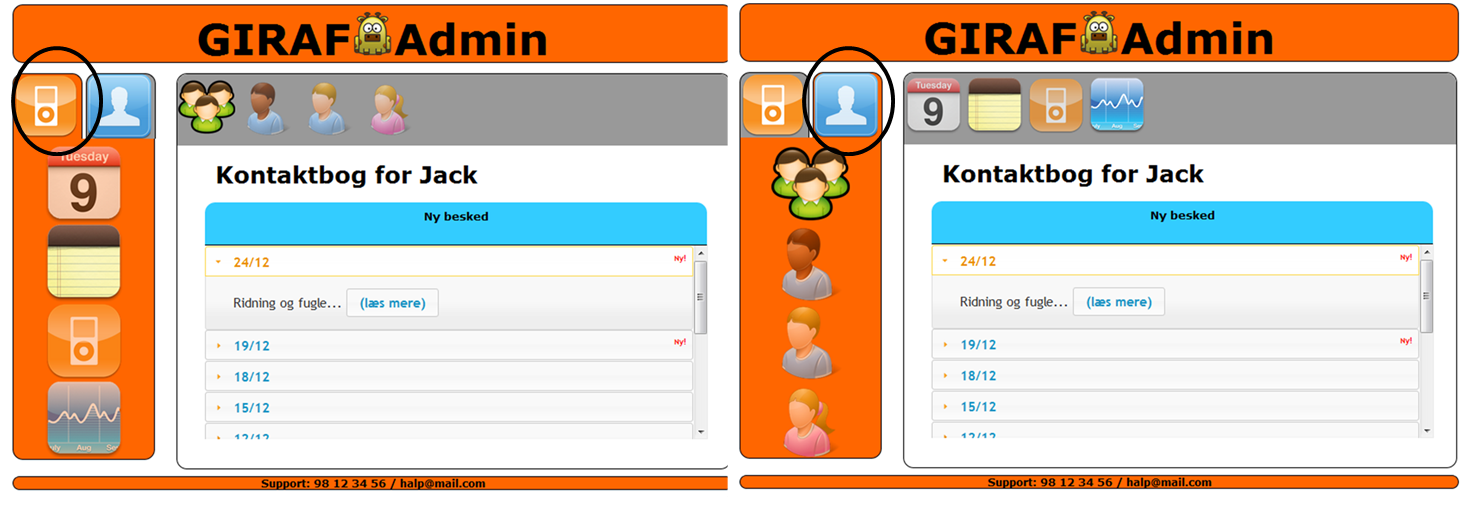
\includegraphics[width=1.00\textwidth]{img/menus.png}
	\caption{The menus in the HTML prototype}
	\label{fig:menus}
\end{figure}


\subsection{Evaluation of the HTML prototype}
In the second interview, see appendix \vref{sec_interview_birken}, with Kristine Niss-Henriksen from Birken we introduced the HTML prototype to her. In general she liked the design but suggested that the icon for a child should be a photo of the child itself, which also was indented. She also expressed a need for a way to reply to a message, which would be useful since it is used both by the parents and kindergarten teachers. Kristine said: ``[communication] \emph{It goes in both directions. The parents write in the contact book in the morning and we write during the afternoon which then can result in a longer dialog between the parties.}'' in appendix \vref{sec_interview_birken} [12:24]. The reply function was then included during the implementation. 

She tried to create a new message and wondered if there was some sort of spell checking in the text field, after realising that this was not the case, she suggested it to be added. We consider this to be a minor improvement, that could be implemented later. 

She saw two versions of the contact book, the first being able to contain several pictures and text; while the other contained text but only one picture - see Figure \vref{fig:createmessage}. She said: "\emph{both can work - because what we do when we are on a trip and add pictures is that we always write something to the picture, but also some general information about the day's events. ... What I think, is that you should somehow be able to separate the text}"\ref{sec_interview_birken} [24:50]. This functionality was added in the contact book during implementation, a text label can be attached to each picture and there is also a text field for general information about the day. 

\begin{figure}[!ht]
	\centering
		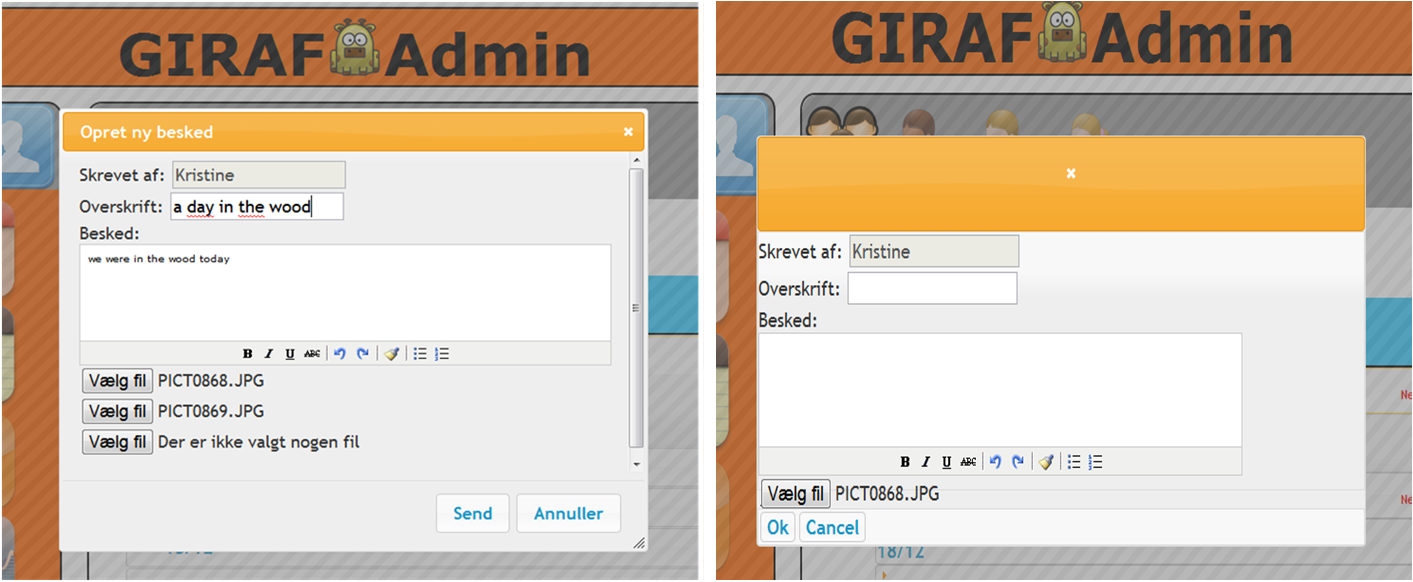
\includegraphics[width=1.00\textwidth]{img/createmessage.png}
	\caption{Create message from the contact book in two versions}
	\label{fig:createmessage}
\end{figure}

In the beginning of the interview, she showed us a standard information sheet that contained the child's name, the parents' name and contact information. The current contact book has this sheet on the first page and Kristine thought that it also should be included in the digital contact book. However, the sheet will not be placed within the contact book.
She also suggested that the information sheet could be implemented as a button among the other applications' administrators, much like the ``Settings'' button, from the first prototype. We chose to place the information sheet among other information about the child in a specific location. 

During the interview she expressed that they rarely edit pictures before printing, but if they were to upload a picture in a message and easily had access to; rotation, crop and resize, she would likely use it. If these ideas were to be implemented, she would also need an undo function. These functions were considered ``nice to have'' and therefore were not prioritised highly in implementation.
From our prototype it was not clear that it would be a closed system, where the kindergarten teachers and parents would have to login before they would be able see or write in the contact book. She considered this to be very important because the information in the contact book might be very sensitive. The Personal Data Protection Act covers this area. 

Kristine pointed out that a child always gets copy of his/hers contact book, when moving out of the kindergarten. If the digital contact book were to be used instead, this tradition would be lost. Therefore she suggested that the user e.g. should be able to print the logs from the contact book so they would not be lost afterwards, since Birken are not allowed to have information indefinitely because of the Personal Data Protection Act. The solution to this problem should be studied further.

After the interview, we wanted to have a start page with general information about meetings and news from Birken to the parents. Kristine first talked about this information in relation to the calendar which is only represented by an icon in the prototype, but that calendar was designed for the child, so the other solution was preferred.

\section{The last paper prototype}
In the last paper prototype, the menu has changed to two vertical menus, where the user needs to click on an application, a child and then press a go-button to get the application settings for that child. This is shown in the Figure \vref{fig:calendar} in which the application aSchedule's administrator for Jack is called, however we never implemented an administrator module for aSchedule. When this design was evaluated, it was considered easier to understand and implement if the user should choose a child or a group of children first and then choose an application. Reason being that the applications' administrator depends on the installed applications on the child's device. The GO-button was considered unnecessary and therefore abandoned, along with the button ``Settings'', as mentioned earlier.

\begin{figure}[!ht]
	\centering
		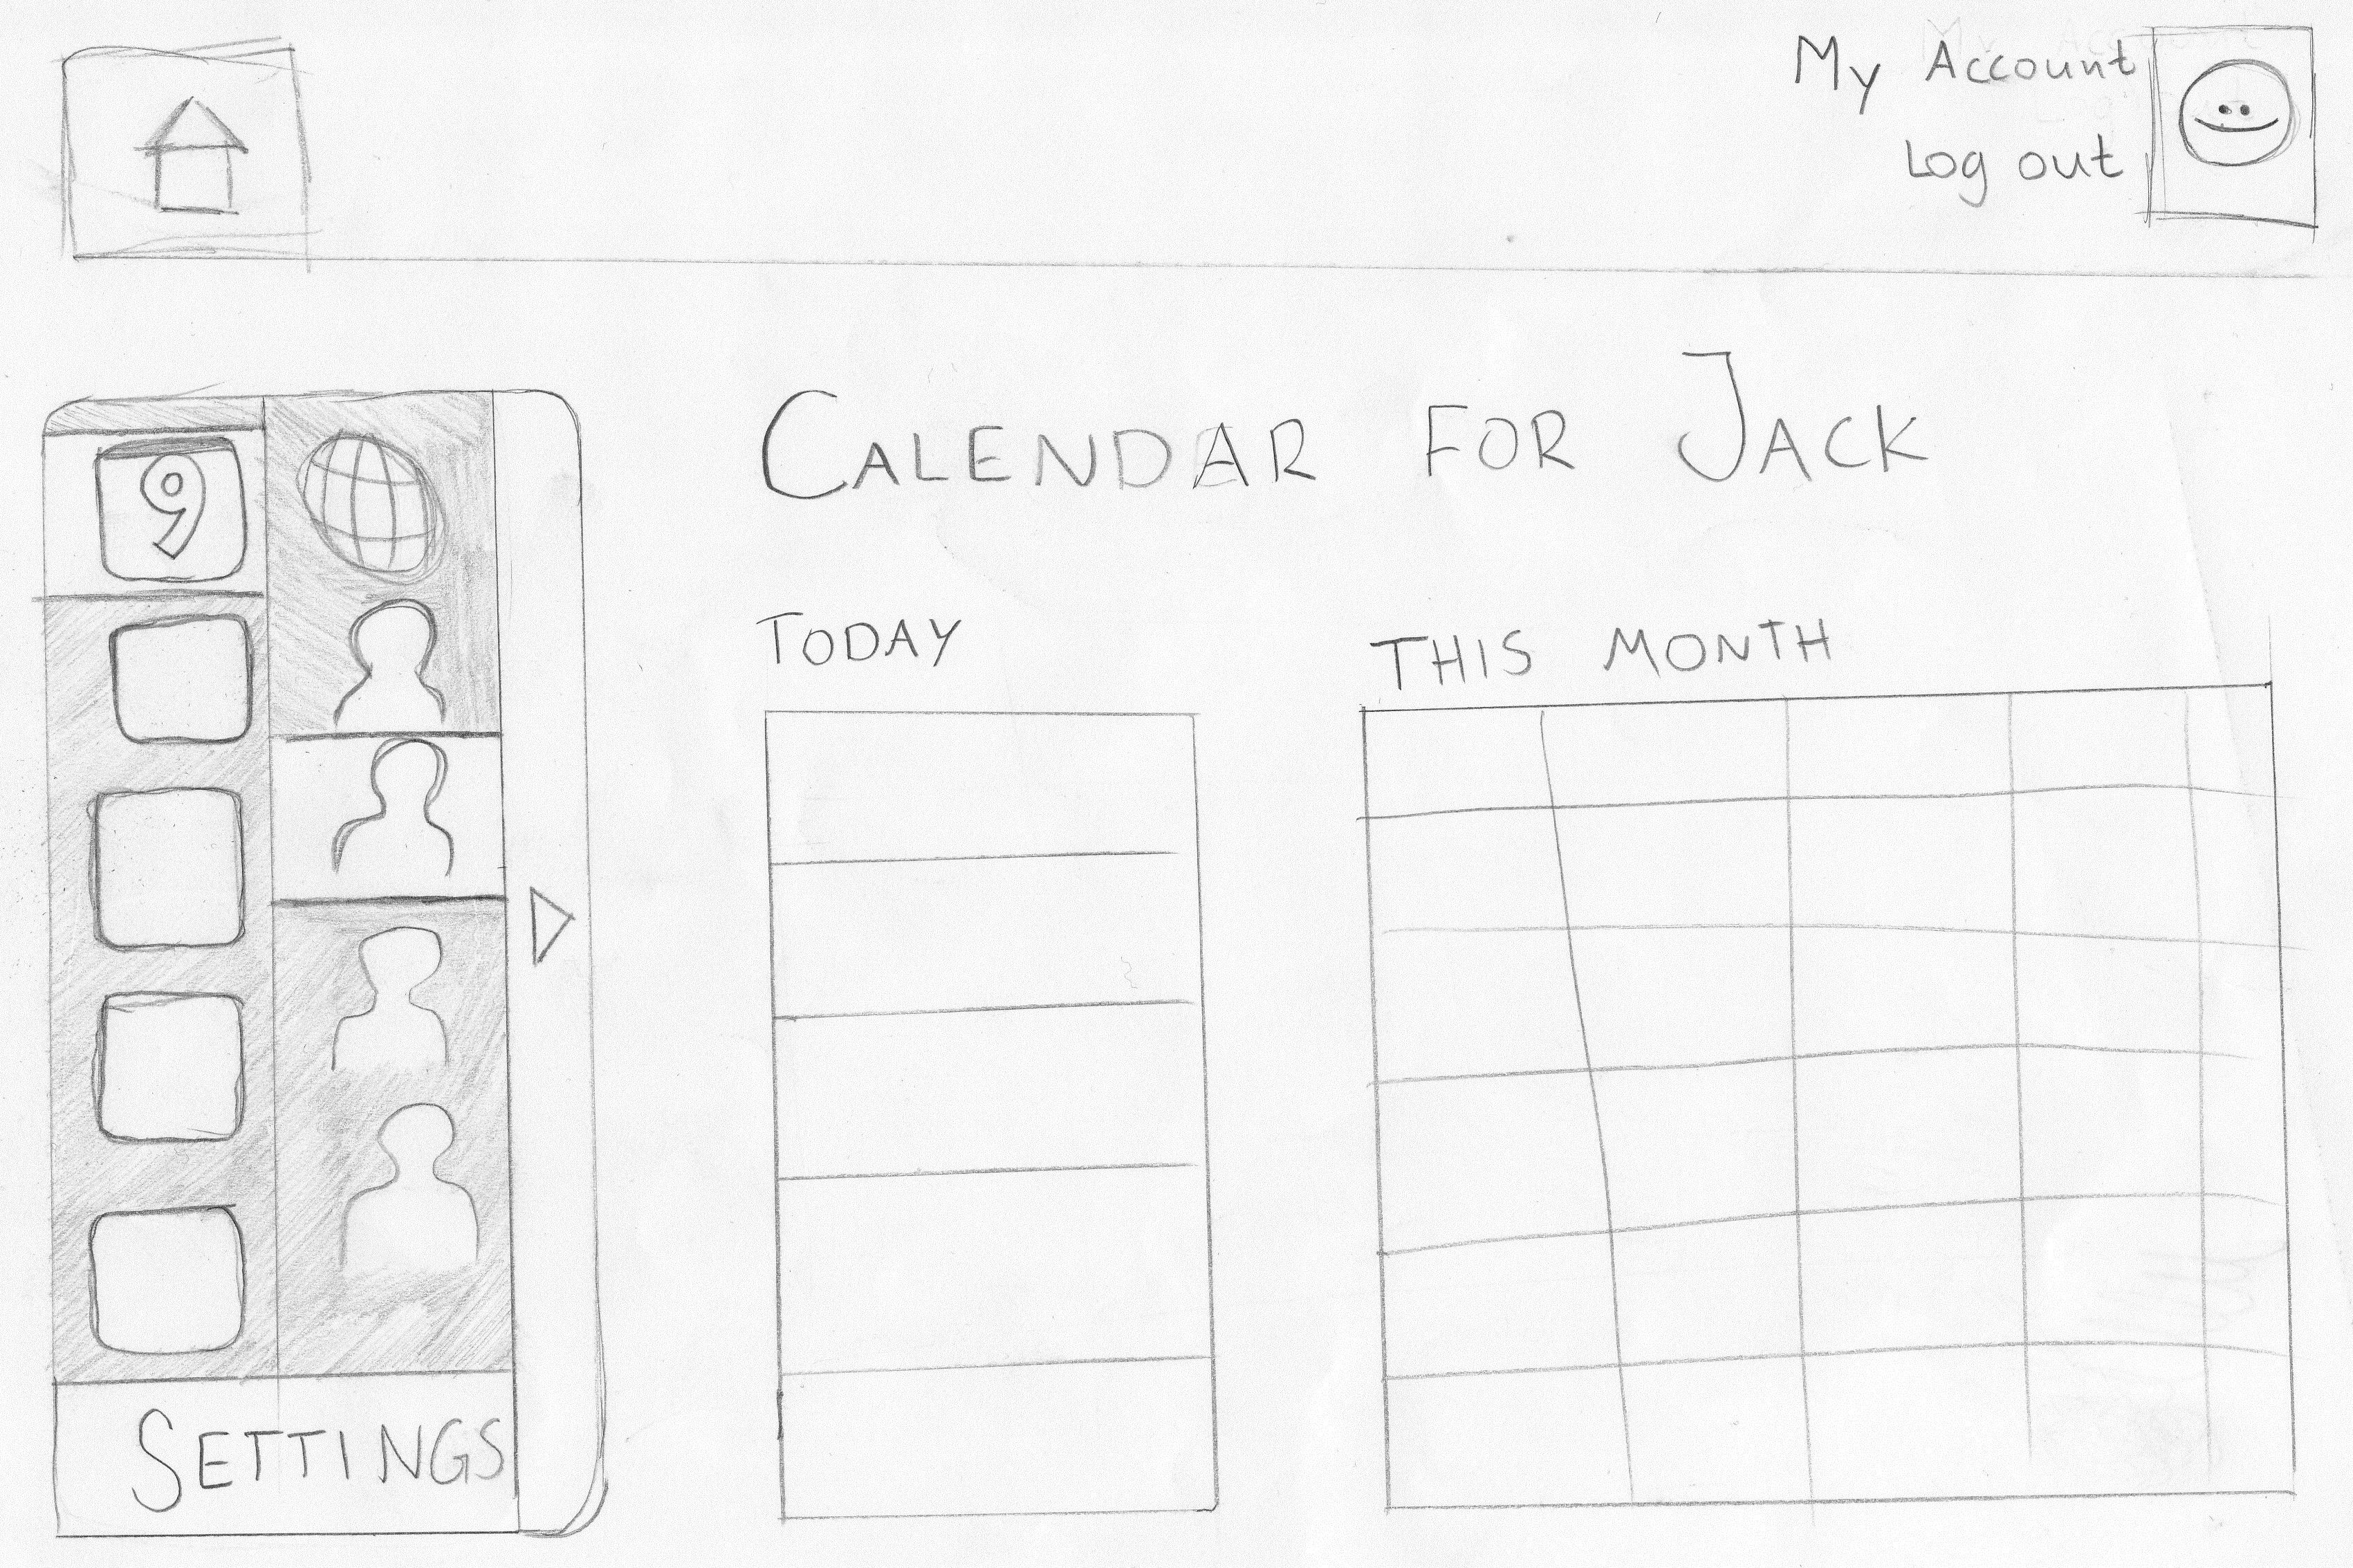
\includegraphics[width=0.60\textwidth]{img/calendar.jpg}
	\caption{Paper prototype of aSchedule's administration application and general design}
	\label{fig:calendar}
\end{figure}

  
In the top-left corner of the prototype is the homepage button which should contain general information and news from the kindergarten, this was one of the changes made as a result of the interview with Kristine. In the top-right corner should be a logout button and a ``My Account'' button, which leads to personal information, shown in Figure \vref{fig:myAccount}. 
\begin{figure}[!ht]
	\centering
		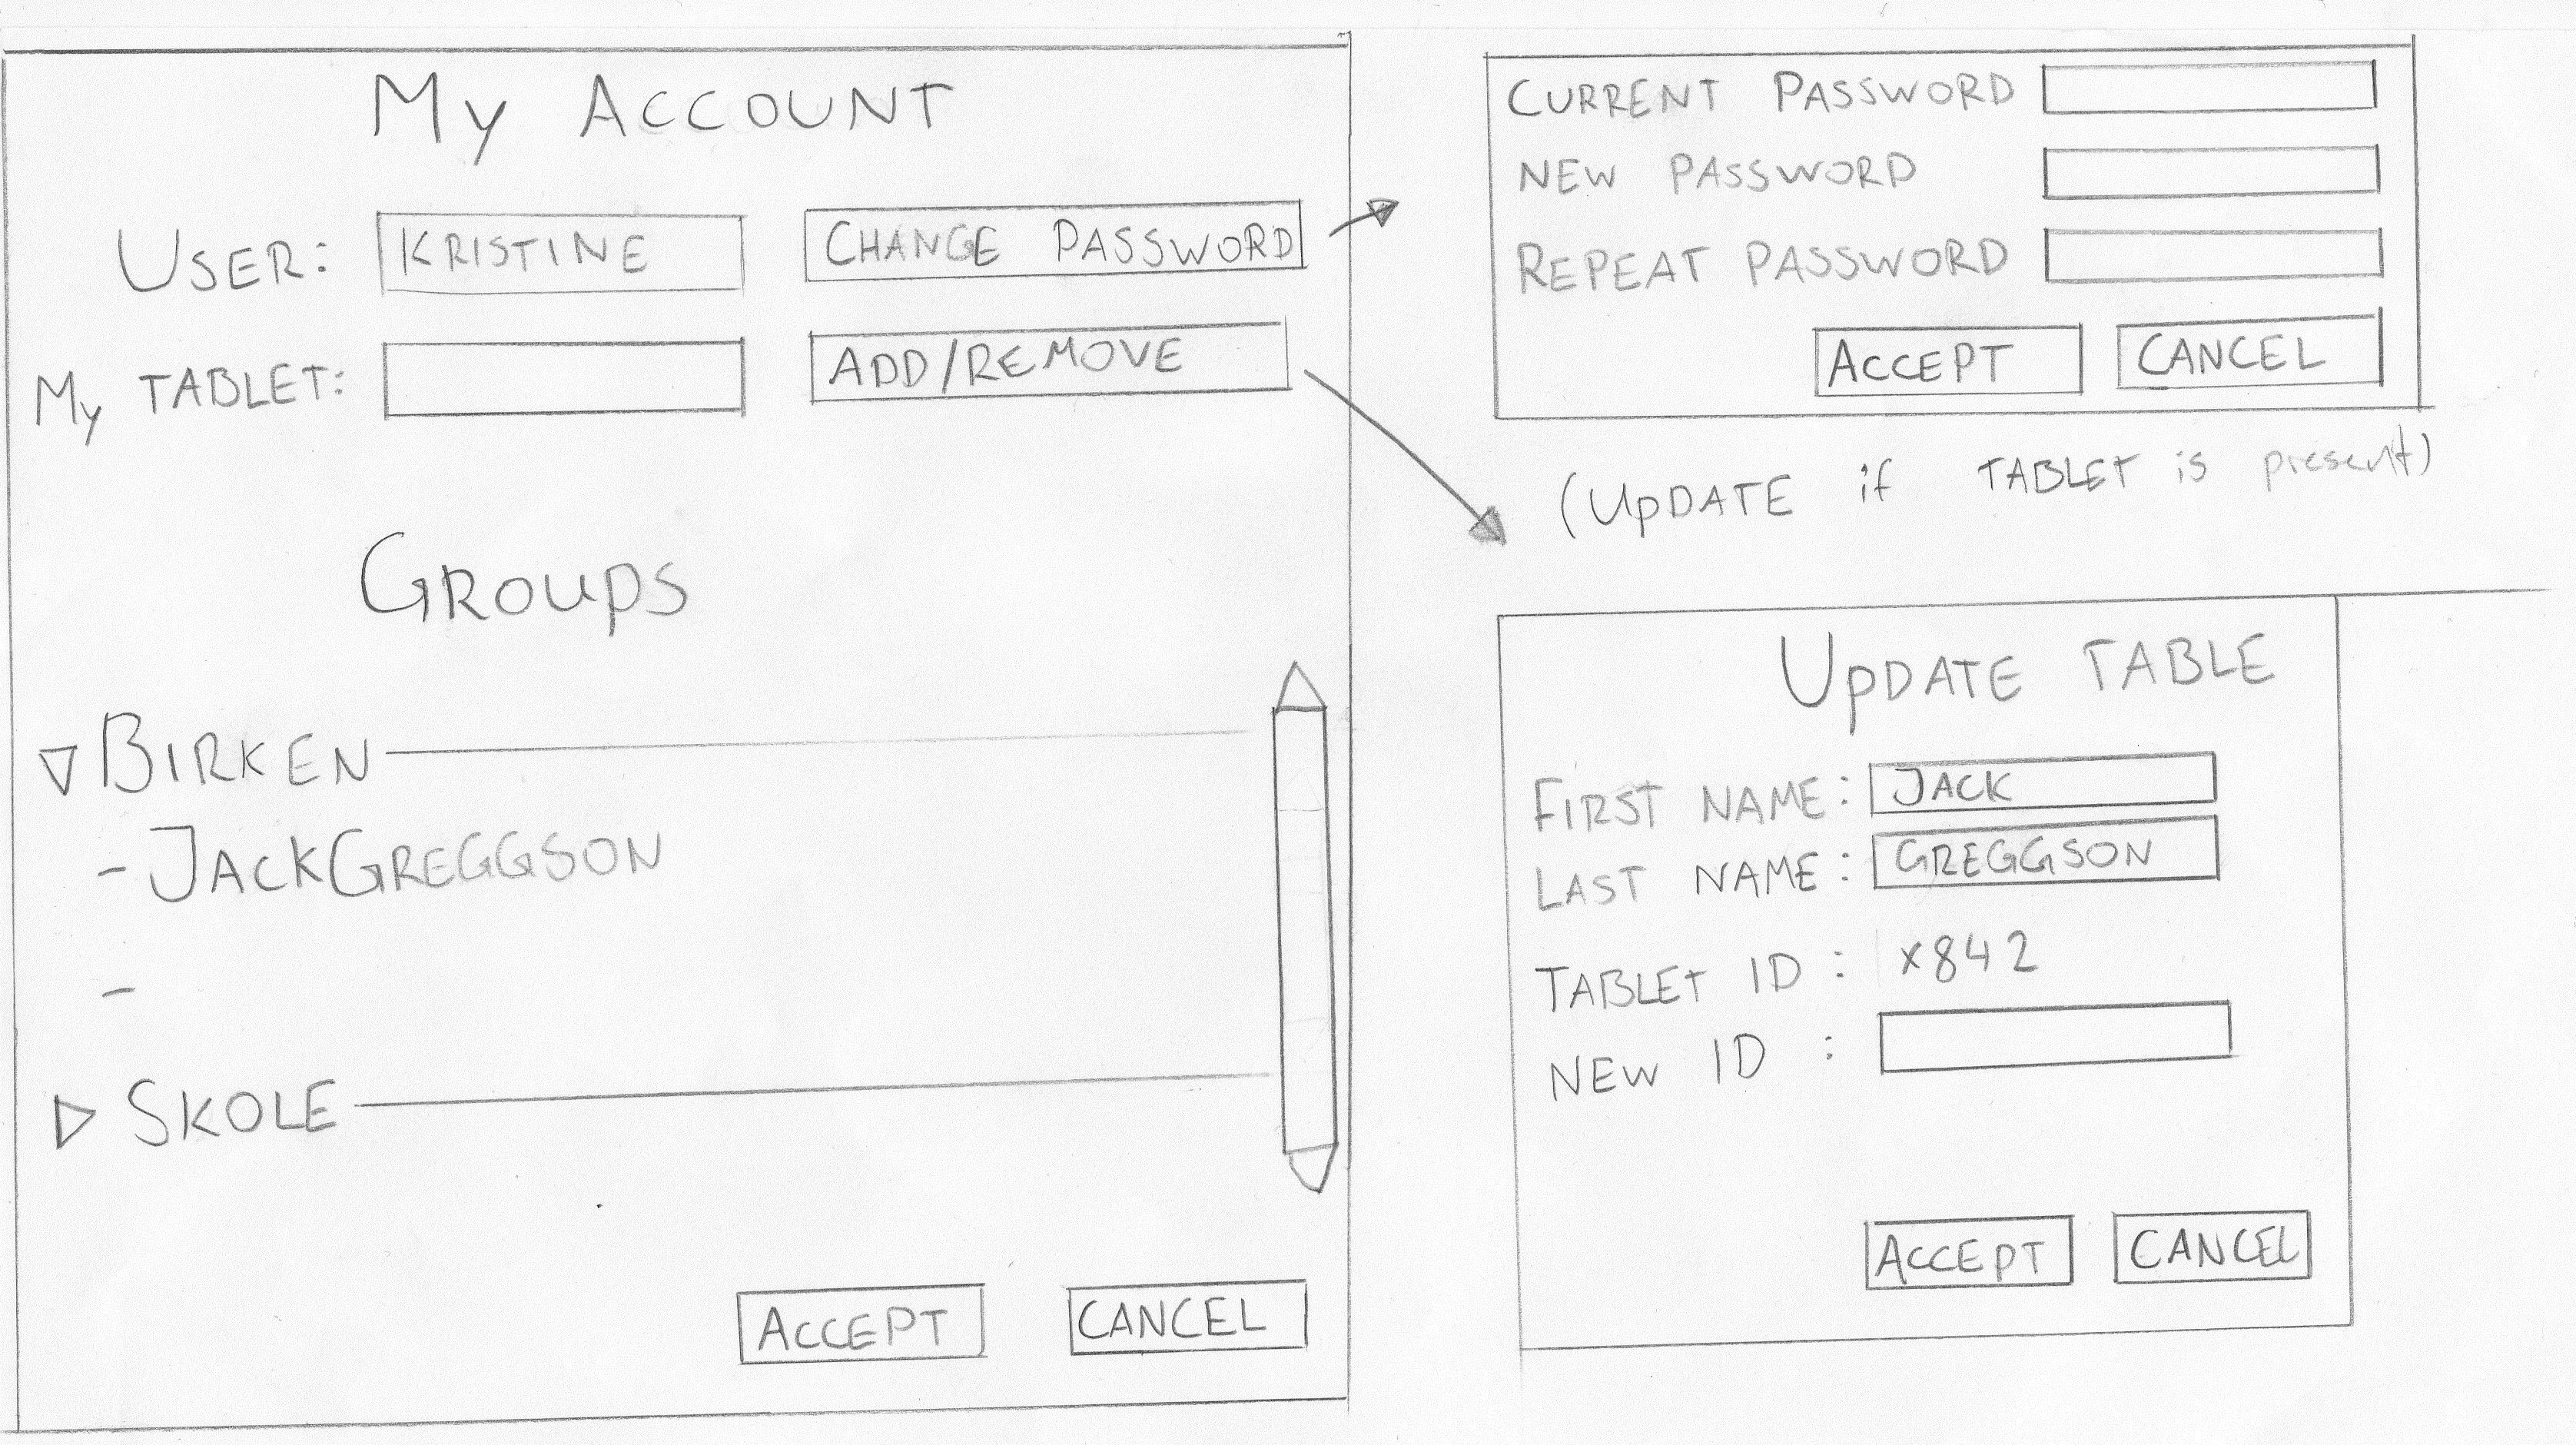
\includegraphics[width=0.60\textwidth]{img/myAccount.jpg}
	\caption{Design of My Account}
	\label{fig:myAccount}
\end{figure}


In this prototype design there is only one page and two pop up boxes, in the first the user can change his/hers password and in the other the user can add/update or delete a device. On the ``My Account'' page the user could also see or update devices in a group, creating confusion. This design was not thought through because the field ``My Tablet'' could be the user's own mobile device. In the beginning it was meant as his/hers child's mobile device and in both cases the user could have more than one mobile device, which should be registered, but is unavailable in this design. 

The group under ``My Account'' is needed because the user of this administration system could both have access to it privately and profecionally. For example the user coud be a parent to an autistic child and also a kindergarten teacher. This mean groups would be necessary when the user wants to change something on all but his/hers child's device without repeating the same process for each device in the kindergarten. The design is missing something that indicates how the user can add a device to a group. In the evaluation of this prototype it was also decided that ``My Account'' also should contain both the child's personal information and device settings. In the implementation it was decided that user information, group, child and child's device should be under different tabs.   
 
\section{The final design}
In the Figure \vref{fig:finalDesign} is the implemented design. It is very similar to the last paper prototype and the HTML prototype. The green menu will contain buttons with pictures and names of the children with connected devices. The pink menu will contain a list of the applications installed on the corresponding child's device. The contact book's design has been altered slightly, this alteration can be seen when the user creates a new message, where instead of opening in a light box window it unfolds when pressing the ``Nyt Indl�g'' label.  

\begin{figure}[!ht]
	\centering
		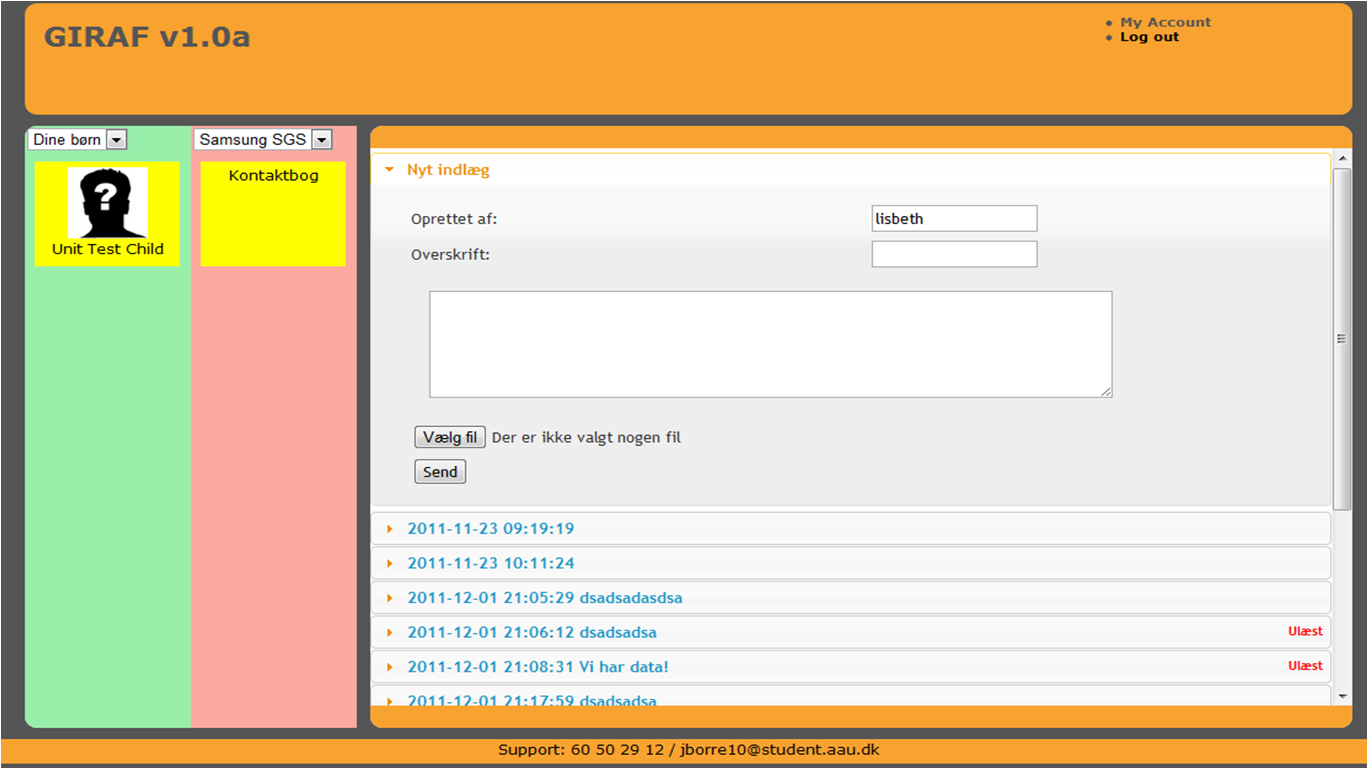
\includegraphics[width=0.90\textwidth]{img/finalDesign.png}
	\caption{Screenshort of the implemented design}
	\label{fig:finalDesign}
\end{figure}


\chapter{Architectural design}
%\section{Class Diagram}
\section{Component architecture}

The architecture of the administration part of the GIRAF system is designed as a client-server architecture. That means that the user uses the client to communicate with the server, where the database lies. Within the client and the server lie three components. These components are called; view, controller and database. These three components communicate with each other through the controller, meaning that controller is the link between the view and the database, which handles calls from both sides. In current design the client does not contain any components, leaving the server with all three; the reason is that the system is 100\% web based and is utilized by means of an internet browser. The component architecture can be seen in figure \vref{fig:architecture}

\begin{figure}[!ht]
\centering
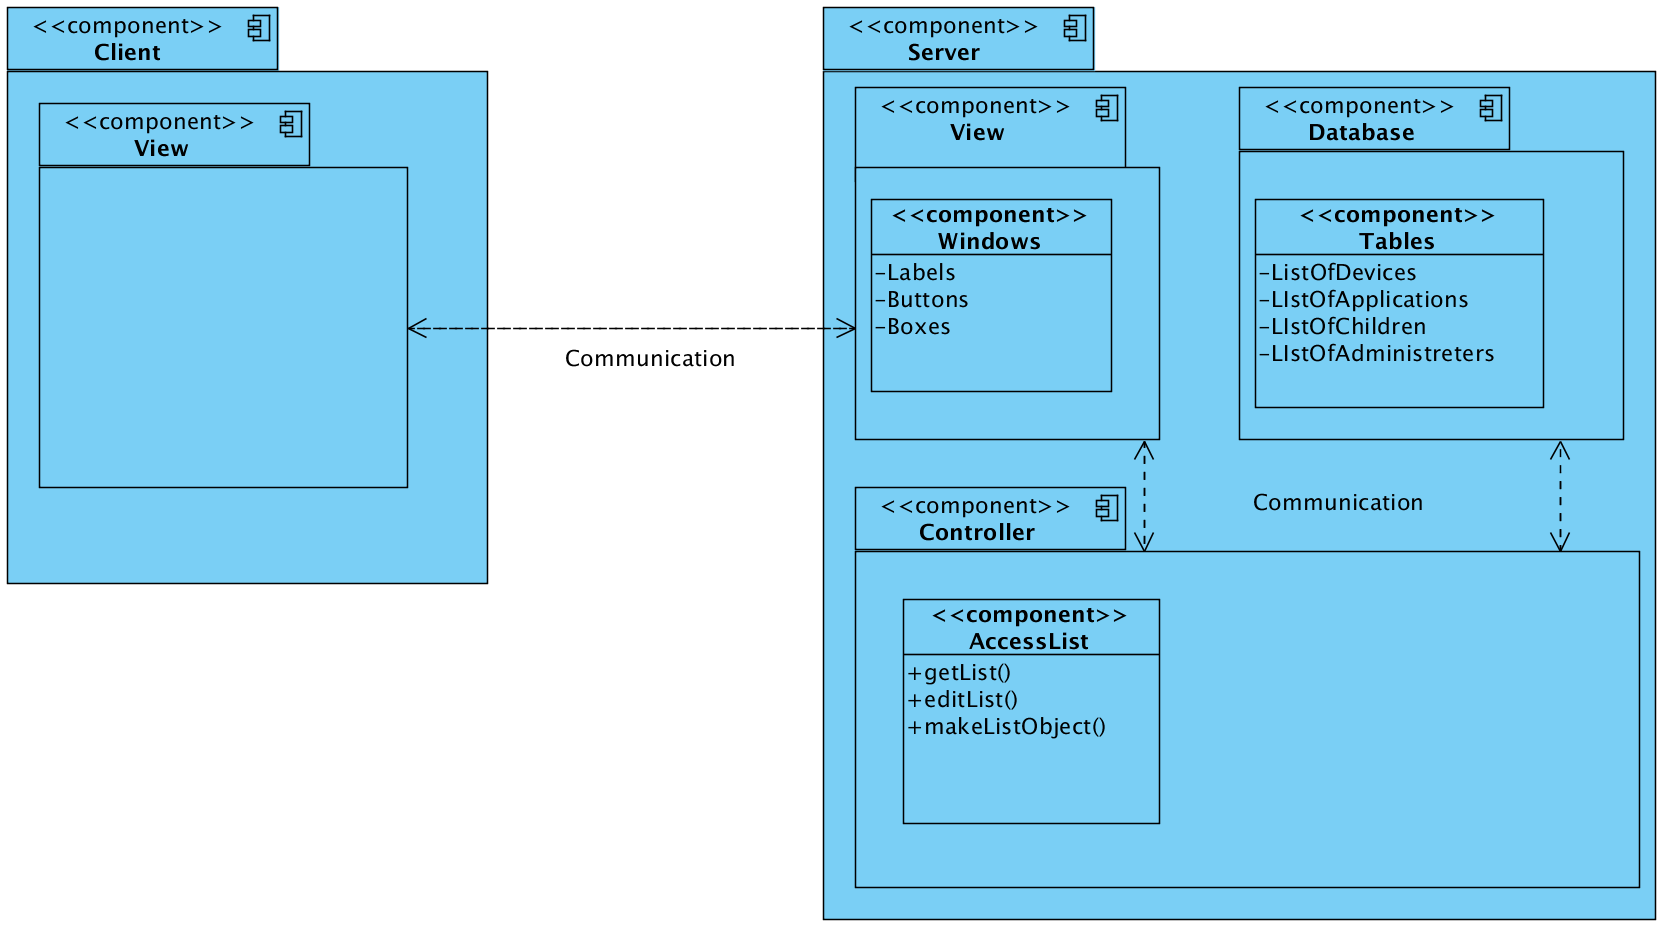
\includegraphics[width=1.0\textwidth]{img/ComponentArketektur.png}
\caption{The figure shows the component architecture of the administrations system}
\label{fig:architecture}
\end{figure}

The three components contain other components, which contain some attributes. These attributes define what function the overall component has, for instance the view component contains a windows component, which contains some attributes called ``labels'', ``buttons'' and ``boxes''. The attributes show that the windows component can contain labels, buttons and boxes.
The controller contains a component with an attribute called \emph{accesList}, this attribute can get a list from the database, edit a list from the database and make an object of a list.
The database contains a component called ``lists'', this component has an attribute which indicates that the database contains lists. Among the lists is a list of devices.
\section{Model-View-Controller}
The model-view-controller (MVC) is an architectural pattern, that separates an application into three parts and has a well defined area of responsibility. First conceived by Trygve Reenskaug in 1979, the architecture's original purpose was to create the illusion of directly manipulating grouped data for the user while still retaining a more effective data model. Beyond this, the clear-cut responsibilities of each component vastly increases maintenance and extension \cite{reenskaug_mvc}
%The model is responsible for all the calculation and data handling, that the controller needs; in fact all the work the application can do is done in the model. The view is the interface that the user interacts with and it is a representation of the model. The controller gets input from the user and is then able to get data or change data from the model, but the controller can also change the view in response to the user input\cite{vmc}. MVC can be used as a framework e.g. to create web applications.

The first iteration of \emph{GIRAF-W-11} followed a more generic three-tier architecture with model, business logic and view. The initial assumption was the view as single interaction point for the user and the remaining architecture as downwards strict. This approach created a very rigid and unextendable structure; that, if extended, created unnecessary complications. There was no central point of access control, views were requested directly by clients and adding functionality (the contact book) proved more a question of hardcoding over flexible adaptation.

Inspired by the web-based MVC frameworks Ruby on Rails (programmed in \emph{Ruby}) and CodeIgniter (programmed in \emph{PHP}), the business logic and view layers were completely remodelled to fit an MVC architecture introducing a central gateway (the \emph{index.php} file) for all user interaction \cite{ci_mvc}\cite{ror_mvc}. Furthermore, user input was delegated to the controller. The benefit is that controllers now determine which view (or views) should be used with a particular request and the same request can result in two very different displays (for example, one fit for small-screen mobile devices and one for wide-screen PC monitors) while business logic remains completely unchanged.

The remainder of this section will discuss the technical design aspects of the three layers individually. For details on final implementations, see chapter \vref{chap_mvc_start}.

% The begin of the design process we used a The Three-tier Architecture with model, business logic and view, however, this created problem in the implementation. Then we decided to use a Model-View-Controller framework because that was more efficient and in the end easier to implement. This decision would also make it easier for future developers to add more functionality, e.g. an aSchudule administrator application. Another advantage of the MVC framework is that the view can be replaced so if Giraf administration application should be displayed on a mobile device then different view could be used.

\subsection{Model}
\label{design_tech_model}
As the foundation on which the entire framework rests, the model needs to be simple to use, yet offering powerful flexibility. The Active Record pattern is an architectural pattern related to relational databases. A database table is represented by a class and a single row of the table as an object of that class. Knowing how a table is usually structured (columns with specific types of data as well as indices determining uniqueness and searchability), the basic class for a record can be defined universally.
In the simplest terms, a single record in a table consists of the following:
\begin{itemize}
    \item One or more fields of data. Each field contains a specific type of data, and may or may not be a null value.
    \item One or more indices connected to the fields. At least one field, the primary key, must be defined.
    \item Zero or more associations with other record types.
\end{itemize}
Some, if not all, of the structure can be analysed from the source database. The SQL standard specifies the INFORMATION\_SCHEMA table containing information about all schemas in the database. Furthermore, several implementations support a DESCRIBE statement simplifying the analysis even more. In essence, a record type's structure can be uniquely determined using only its source table.
The final result is a single class that requires minimal effort to inherit in specialisations (only changing the source table), leaving later designers to focus solely on the properties that make a particular specialisation unique.

\subsection{Controller}
As the next immediate layer after the model, the controller is best described before the view (in contrast to the literal name of the architecture).
% Discuss how designing a triad of controllers - primary, secondary and supporting - makes sense from the point of view of security, control and extendability. Clearly defined roles give clearly defined types of output.
From MVC certain aspects of the controller are clear. Examples of functions for the controller can be seen in figure \ref{fig_controller_cb}. It must receive user input and affect changes in the model depending on said input. It should also instruct the view layer to display the correct/relevant output to the user.
Beyond this there are no restrictions on how the controller should relate (in structure) to the model or view. For example, there are no demands that a specific part of the model reside in a 1:1 relationship with a particular controller. Indeed, a strength of the design is the controller's mandate to create an amalgam from the model that fits the situation for which it was created.
From a technological standpoint, the controller - as the point for user input and origination of output - could be considered the only exposed element of the server that GIRAFAdmin resides on. Birken has earlier stressed the need for absolute security in the implementation (particularly in regards to personal information and images), and creating a virtual bottleneck in resource availability should result in a degree of control sufficient for these purposes.
Finally, the specific controllers necessary for the current specification can be discerned. The controllers should be designed around certain contexts, and given the function list created during the early design process works as an indicator. As an example, the functions defined for the contact book have several similarities to \emph{CRUD} (for more information see \vref{CRUD}), the basic functions of database storage.

\begin{figure}[ht]
	\begin{itemize}
		\item Create new message
		\item Create reply
		\item Attach image
		\item Show a message
		\item List messages
	\end{itemize}
	\caption{\label{fig_controller_cb}Function list for contact book controller.}
\end{figure}

\subsection{View}
MVC specifies that the view needs to reflect changes in the model, but does not explicitly define when the view is updated.
The controller determines which view will fit a request and instructs the view in what to display, typically by passing it a subset of the model pertaining to the request. This suggests that views be designed according to two axis: the client type (text-based, mobile device, PC, and such) and the content type (more specifically, tailored to the controller most likely to invoke the view). While the controller determines which view to display, the question of how (or when) state changes in the model are shown remain undetermined in the MVC model. The two base options are using either the observer pattern, updating the view by request of the model whenever states change, or the polling pattern, updating the view only when this is explicitly requested. Choosing an approach is more a question of prudence in accordance with the available technology than considering the resulting system complexity. In order to make a decision it is necessary to delve, briefly, into the target domain of web software. HTTP is, by definition, a system of action-reaction. A client will never be affected to perform actions from remote sources, effectively limiting input to go outwards (client to server) and output inwards (server to client).

For the sake of argument, consider the contact book, and the user requesting a list of relevant messages. The client requests a list from the server and the appropriate view is invoked, rendered and returned. If, after the page is loaded, someone creates a new relevant message for the user, the server has no direct way of iniating a change in the view.
It is possible to create the effect of an observer pattern by using timed polling client-side. Implementing JavaScript logic into the final view would instruct the client to poll the server for changes at regular intervals, updating the view as necessary. However, this is a feature unique to the view and does not create the observer connection sometimes detailed between model and view. Instead, it stresses the necessity for views to be largely self-contained where possible.

The conclusion of this is that views need to be built within the contexts of purpose and target platform with the understanding that they must implement an active polling component if state changes need to be reflected without direct user interaction.
% Debate that in a web-server context, designing views to work as polling devices and not observers is a proper consideration.

\chapter{Android-Server synchronization}
\label{androidDesign}
This chapter deals with the design of the Android Application framework, which provides information on how to implement a protocol, a client and server for synchronization of GIRAF applications, user profile and settings. However, this was not fully implemented. 
\section{GIRAF synchronization framework}

The original project proposal was about creating an administrative PC tool which should be able to synchronize data for a GIRAF mobile device. This could be one device at the time, or many devices through a centralized management system. In the beginning of the design process this general idea was used and developed upon. From this, specifics to a solution was made, including a detailed design process, additions to the existing framework and some proof-of-concept code. After the 2 first interviews with Birken, this part of the project was discontinued, because the contact book application was a more useful to them\vref{first_interview_birken}. Although it was discontinued, some of the code parts are fully functional; and it is still an important part of some of the initial project work that was made. Furthermore, the source code and designs made here, could be carried on as material for further development. 

The original project proposal was about creating an administrative PC tool which should be able to synchronize data for a GIRAF tablet device. This could be one device at the time, or many devices through a centralised management system. In the beginning of the design process this general idea was used and developed upon. From this, specifics to a solution was made, including a detailed design process, additions to the existing framework an some proof-of-concept code. After the two first interviews with Birken, this part of the project was discontinued, because the contact book application was a more useful to them (see \vref{first_interview_birken}). Although discontinued, some of the code parts are fully functional; and it is still an important part of some of the initial project work that was made. Furthermore, the source code and designs made here, could be carried on as material for further development. 


The general idea included that the software should support user profile and application settings synchronization. Moreover, the existing GIRAF-android client has functionality to install and view available applications. In milestone 1.0 of the client software, this feature should be merged with the synchronization application, making it possible to control available applications through an Access Control Lists (ACL).

\section{Protocol design v0.1 draft}
This design has not been fully implemented, only some of the design parts have been written in code. It also contains milestone perspectives; some features are planned in the first milestone release (version 1.0) and a short description on which functionality that should be implemented follows. In general; protocol milestone functionality is described in detail and can be used as a direction indicator for further development.  

\subsection{Handshake}
The first message sent from the client is a handshake. The handshake is very simple, since it only expects a string containing ``HELLO'', immediately followed by a version string.

\subsection{Version} 
The version string consists of 3 parts of version numbers, which indicates the significance of changes made to the software. First number is major release, next is minor release, and the last number is the build number. The version numbers are separated in the string by a dot (".") character, example for a version string would look this: "1.0.1". If the server encounters a client with a newer version than its own, the server will at the moment refuse the client to connect. However, theoretically, the server could still offer functionality that has not been changed in the new version, or which does not have updated dependencies. In protocol milestone 1.0 this is not planned; however, such functionality could still be implemented by sending a short version string together with the message making it possible for the server deciding whether a particular function is still supported, even though the client version is newer. However, such scenario is unlikely to happen. 
If a valid version is detected, the server answers "OK" and command messages can now be sent from the client.

\subsection{Ident}

The ident is sent to the server after the client receives the "OK" signal. After an ident is successfully received by the server, the server sends an "OK" signal to the client, indicating that it is ready to receive further instructions. 

Ident is performed after a successful handshake and version check - and the client have received an "OK" from the server - the client will create an MD5 hash of its WiFi (Wireless Fidelity) unique network address, also called a Media Access Control address (MAC). MAC addresses are generally used to identify network equipment of any kind using any implementation of the IEEE 802 standard\cite{IEEE}, and are frequently used to control network equipment through an ACL\cite{cisco}. The purpose of the ident is to create a simple, yet effective ACL which provides a filter on which application settings (and, in protocol milestone 1.0 this will also include installable applications) are accessible to the client. MD5 hashes are not collision-safe\cite{ACCESSDATA}, %ville �nske at parantserne forsvandt
but any collisions would be highly unlikely, due to the source, which in this case is MAC-48 address. 
The ident is sent to the server after the client receives the "OK" signal. After an ident is successfully received by the server, the server sends an "OK" signal to the client, indicating that it is ready to receive further instructions. 

\subsection{Timestamp}
After a successful ident, the client sends a timestamp string of the current time formatted as unix time. The server then calculates the difference between its own time and the client's time, taking into calculation that the server and client might be in different time zones. If the time difference is greater than +/- 12 hours, which is the max possible difference when calculating time, the server returns an error message "TIME\_NOT\_CONFIGURED" to the client, and ends communication. Otherwise, the server answers "OK". 
Next, the client sends it's last update time to the server. If no update time exists, the server receives the "FIRST\_UPDATE" message from client.

\subsection{User profile transfer}
The client initiates the user profile transfer  by sending the "USER\_PROFILE" command message. If the server receives the message, an "OK" is returned to the client. The client sends any timestamps newer than the last update time. If an update from the server is newer than the last update time, and the client has a conflicting update, the server always wins. All data with a newer timestamp is transmitted back to the client. When all data has been sent, the server sends the "DONE" signal. 

\subsection{Application transfer}
Application transfer is initiated by the client sending the "APP\_TRANSFER" command message to the server and the server responds with "OK". The client sends a list of installed GIRAF applications together with the application version string. If any updates are available, these will be installed first. Any marked applications for installation will be sent to the server after the application updates are completed.   

\section{Settings transfer}
Initiated by the client, by sending the ``SETTINGS\_TRANSFER'' message to the server. The client locates all rows in the local SQLite database with a newer timestamp than the last update time and transfers these rows the server. The server evaluates each row against the centralized database. If a newer entry already exists in aforementioned database, the data is dropped - in other words, server always wins when data collision occur. This choice makes sense, since the device administrators pushing updates should be ensured that new settings reaches the target device; An example could be a newly installed application - which haven't been updated - containing database information, where the user only has read-only access. This ensures that device administrators still retain the possibility to update the values.

When all data has been successfully sent, the client sends the ``OK'' message - next, the server sends back any rows that is newer than the last update time. Although not planned in milestone 1.0, the ability to implement group settings for applications should be kept in mind if such functionality is needed in the future. 

The version string consists of 3 parts of version numbers, which indicates the significance of changes made to the software. First number is major release, next is minor release, and the last number is the build number. The version numbers are separated in the string by a dot (``.'') character, example for a version string would look this: ``1.0.1''. If the server encounters a client with a newer version than its own, the server will at the moment refuse the client to connect. However, theoretically, the server could still offer functionality that has not been changed in the new version, or which does not have updated dependencies. In protocol milestone 1.0 it is not planned; however, such functionality could still be implemented by sending a short version string together with the message making it possible for the server deciding whether a particular function is still supported, even though the client version is newer. However, such scenario is unlikely to happen. 
If a valid version is detected, the server answers ``OK'' and command messages can now be sent from the client.

\subsection{Ident}

The ident is sent to the server after the client receives the ``OK'' signal. After an ident is successfully received by the server, the server sends an ``OK'' signal to the client, indicating that it is ready to receive further instructions. 

Ident is performed after a successful handshake and version check - and the client have received an ``OK'' from the server - the client will create an MD5 hash of its WiFi (Wireless Fidelity) unique network address, also called a Media Access Control address (MAC). MAC addresses are generally used to identify network equipment of any kind using any implementation of the IEEE 802 standard\cite{IEEE}, and are frequently used to control network equipment through an ACL\cite{cisco}. The purpose of the ident is to create a simple, yet effective ACL which provides a filter on which application settings (and, in protocol milestone 1.0 this will also include installable applications) are accessible to the client. MD5 hashes are not collision-safe\cite{ACCESSDATA}, but any collisions would be highly unlikely, due to the source, which in this case is MAC-48 address. 
The ident is sent to the server after the client receives the ``OK'' signal. After an ident is successfully received by the server, the server sends an ``OK'' signal to the client, indicating that it is ready to receive further instructions. 

\subsection{Timestamp}
After a successful ident, the client sends a timestamp string of the current time formatted as unix time. The server then calculates the difference between its own time and the client's time, taking into calculation that the server and client might be in different time zones. If the time difference is greater than +/- 12 hours (The max possible difference when calculating time), the server returns an error message ``TIME\_NOT\_CONFIGURED'' to the client, and ends communication. Otherwise, the server answers ``OK''. 
Next, the client sends it's last update time to the server. If no update time exists, the server receives the ``FIRST\_UPDATE'' message from client.

\subsection{User profile transfer}
The client initiates the user profile transfer  by sending the ``USER\_PROFILE'' command message. If the server receives the message, an ``OK'' is returned to the client. The client sends any timestamps newer than the last update time. If an update from the server is newer than the last update time, and the client has a conflicting update, the server always wins. All data with a newer timestamp is transmitted back to the client. When all data has been sent, the server sends the ``DONE'' signal. 

\subsection{Application transfer}
Application transfer is initiated by the client sending the ``APP\_TRANSFER'' command message to the server and the server responds with ``OK''. The client sends a list of installed GIRAF applications together with the application version string. If any updates are available, these will be installed first. Any applications marked for installation will be sent to the server after the application updates completes.   




\section{Client design}
The client is designed as a local service based upon the Remote Messenger Service Sample provided by the Android development community\cite{AndDevel3}, which unlocks some features of the android subsystem. An example would be the ability to send notifications to the user and place them in the android notification bar.

The client starts together with the GIRAF Launcher on the device and pulls the server for updates with a frequency of 30 minutes. This frequency has been chosen due to extend the battery-life of the Android device. However, even though it is not a planned feature, the push functionality would greatly lower battery consumption. In some scenarios it is likely to imagine that many hours will pass before any updated data will be needed to be synchronized. To save battery life, and to receive updates as they get posted, such functionality could be implemented. It is not planned in milestone 1.0 since it is not a critical feature for the system to work properly since it primarily is an optimization and does not add any extra functionality at this moment. 


It has earlier been speculated that from the way SQlite works, issues with many applications accessing the same SQlite database might resort in database errors. However, in SQlite version 3.0.0 new locking features were introduced making it possible to let the system control when exclusive locks occur - which is used when writing to the database - through a pager module\cite{SQlite}. Since all newer Android Operation Systems ships with SQlite 3.4.0 or newer\cite{AndDevel} this problem is not as big as it used to be. However, GIRAF application developers should still minimize the needs for reserved and exclusive locks, to prevent the client from getting the SQLITE\_BUSY error.   

The current GIRAF client already contains functionality to fetch and install applications from the GIRAF Place application server, this functionality is planned to be extended with an update feature, where the synchronization service pulls the server for updates making it into an automated process. This could be extended to include remote installation of applications on the device which Android currently features. Inspiration on how such features could be implemented using the Android service class is accessible \cite{DevRemote}. Moreover, the client handles database writes. It has earlier been speculated that from the way SQlite works, issues with many applications accessing the same SQlite database might resort in database errors. However, in SQlite version 3.0.0 new locking features were introduced making it possible to let the system control when exclusive locks occur (Used when writing to the database) through a pager module\cite{SQlite}. Since all newer Android Operation Systems ships with SQlite 3.4.0 or newer\cite{AndDevel} this problem is not as big as it used to be. However, GIRAF application developers should still minimize the needs for reserved and exclusive locks, to prevent the client from getting the SQLITE\_BUSY error.   


\subsection{Message handling documentation}
This section deals with the documentation of signal messages the client receives from the server - make note that the server will never send any command messages; the client interprets the signals sent from the server and executes functions as needed.   

\begin{description}
	\item[OK] Everything is ``OK''. The client waits for this signal before sending more data. Also used for debugging; in milestone 1.0 unnecessary OK messages can be removed from the transfer processes. 
	\item[DONE] Signal message received at the end of a successful settings, user profile or application transfer.
	\item[KTHXBYE] Signal message that terminates communication. Logs the current time as update time. This message is only received after a complete synchronization has completed.
	\item[TIME\_NOT\_CONFIGURED] The ``TIME\_NOT\_CONFIGURED'' string is handled by the client by placing a notification in the Android notification bar. If the notification is pressed, it will open up the date/time configuration page in Android Settings.
\end{description}

\section{Server design}
The server handles communication with the MySQL server backend and receives instructions from the client in the form of command messages. The current \emph{giraf\_web server project} has been migrated, such that only 1 server application exists. 

\subsection{Message handling documentation}
This section deals with the documentation of signal messages the server receives from the client.  


\textbf{FIRST\_UPDATE}\\
Message sent by client when the first update occurs, which usually occurs right after the device is turned on for the first time and user profile has been completely filled out or when a factory reset has occurred.\\

\textbf{SETTINGS\_TRANSFER}\\
Message received from client initiating settings transfer. \\

\textbf{USER\_PROFILE}\\
Message received from client initiating user profile transfer. \\ 

\textbf{APP\_TRANSFER}\\
Message received from client initiating application transfer. \\

\textbf{OK}\\
A message is sent to the server, that indicates everything is "OK" and the server waits for this signal before sending more data

\textbf{FIRST\_UPDATE}\\
If this message is received, the server knows that this is a new device - or if the device already exists in the server database - a factory reset has been performed.
If a factory reset has been performed, the server immediately starts to synchronize data, by sending the user profile first, application list second and application settings last. Between each step, the server waits for an "OK" message from the client. 

\textbf{BYE}\\
Command message ending communication. 

\begin{description}
	\item[FIRST\_UPDATE] Message sent by client when the first update occurs (Usually right after the device is turned on for the first time and user profile has been completely filled out) or when a factory reset has occurred.
	\item[SETTINGS\_TRANSFER] Message received from client initiating settings transfer.
	\item[USER\_PROFILE] Message received from client initiating user profile transfer.
	\item[APP\_TRANSFER] Message received from client initiating application transfer.
	\item[OK] A message is sent to the server, that indicates everything is ``OK'' and the server waits for this signal before sending more data.
	\item[FIRST\_UPDATE] If this message is received, the server knows that this is a new device - or if the device already exists in the server database - a factory reset has been performed.
If a factory reset has been performed, the server immediately starts to synchronize data, by sending the user profile first, application list second and application settings last. Between each step, the server waits for an ``OK'' message from the client. 
	\item[BYE] Command message ending communication. 
\end{description}


\section{Implementation extensions to the GIRAF Framework}
A few extensions had to be made to the GIRAF framework in order to get the functionality needed to make a successful synchronization, since only a few parts were fully implemented, only those that reached a final state will be discussed here. 

\subsection{Sw3SqliteToClass - addition to the sw6.library package}
The Sw3SqliteToClass package contains functionality to fetch all data from the sqlite database. The commands can be modified such that only data with a specific timestamp gets returned. The additions were made in its own package due to the design philosophy that only minor changes should be made to existing code created by the SW6 groups.

This particular code stub returns the timestamp for specific application, a specific variable and a specific datatype:

\lstset{language=JAVA}
\begin{lstlisting}
public static Cursor getSettingTime(Context context, String appName, String varName, String dataType) throws SettingNotFoundException 
{
		Uri settingRequest = Uri.withAppendedPath(PrivateDefinitions.CONTENT_URI, dataType + "/" + appName + "/" +  varName + "/" + PrivateDefinitions.TIMESTAMP);
		Cursor settingCursor 	= context.getContentResolver().query(settingRequest, null, null, null, null);	
		return settingCursor;
}
\end{lstlisting}

The client can pull a list of installed applications by creating a new instance of the Android \emph{PackageManager} class and call the \emph{getInstalledApplications(int flags)} method\cite{AndDevel2}.

\chapter{Conclusion}

By making diagrams, following patterns and splitting the system into different parts, designing the system has been trivial.
When designing it was crucial that the group kept redesigning and improving the prototype, got feedback from outside and visualised more than just the interface which the user interacts with.
Redesigning the prototypes helped the group to better understand the mistakes made on previous ones.
The feedback from the group's contact helped make final decisions and bring focus on to more important parts of the system.
While the interface is extremely important when designing, the also important components that make the system functional were not forgotten.
After visualising, prototyping and designing the architecture of the system, implementation of the final product began.



% 3. Implementation
\part{Implementation}

\chapter{Tools \& Languages}
\label{implementation_tools_languages}
\section{Designing tools}
For development of the system, four tools were used, the markup language \textit{HTML} along with the style sheet language \textit{CSS}. And then \textit{PHP} and \textit{JavaScript}, both scripting languages. These are some of the most common web-design tools and have easy-access documentation. All four are currently supported by the most common browsers, including but not limited to \textit{Google Chrome}, \textit{Mozilla Firefox} and \textit{Internet Explorer}.
The reason for so many tools is the difference in functionality, \textit{HTML} provides the browser with information about how to build a website, along with \textit{CSS} that defines the structure, layout and general styling. \textit{PHP} and \textit{JavaScript} have provide functions and data-manipulation that markup languages do not provide.
\cite{html}\cite{css}\cite{php}\cite{javascript}

\subsection{HTML \& CSS}
\textit{HTML} is an acronym for HyperText Markup Language. With elements, the building blocks of \textit{HTML} one can create a website exclusively with text, layout, images and more, although \textit{CSS} is recommended for layout and styling. \textit{CSS} is an acronym for Cascading Style Sheets and is designed primarily to separate the website contents from the presentation.
What \textit{CSS} provides with the separation is structure and readability for the developers since the code itself is not visible to the users and \textit{CSS} provides no extra functionality.\cite{html}\cite{css}

\subsection{PHP}
\textit{PHP} is an acronym for PHP: Hypertext Preprocessor and is a server-side scripting language. As the name inclines, it is preprocessed, on the website server, to automatically write \textit{HTML} code. In other words \textit{PHP} is used to generate results displayed in \textit{HTML}. While \textit{PHP} can run recursive functions, generate code and transport data, it is static in view, all the work is handled by the server hosting the website, which then only displays results. To develop dynamic web content, \textit{JavaScript} or equivalent is needed, which brings us to the next section.\cite{php}

\subsection{JavaScript}
\textit{JavaScript} not to be confused with \textit{Java}, is a scripting language that provides dynamic web content. That is able through client-side execution of web related scripts. The browser gets instructions from the website about how to execute the proposed content, where it is the user's choice of whether to run these instructions.
Since most browsers support dynamic web content through \textit{JavaScript} execution, many developers run scripts on their websites to increase the visual aspect of the website and to make dynamic checking of forms and spelling for example.\cite{javascript}

\chapter{Model, view and controller}


\section{Overview}
\section{Implementation of Model-view-controller}
In Figure \vref{fig:overview} is an overview how our model-view controller framework/architecture has been implemented in our application where the arrows are call dependencies. It is an incomplete representation for the program because not all classes have been included in the figure, however, all the connections between the controller and model's classes are represented. 

In the figure the Model's seven classes, sql\_helper excluded, are all used by at least one controller while the sql\_helper is used by the other classes to relay SQL commands to the database. The model will be further explained in section \vref{model}. All in all six views have been implemented (header, footer and four pure "content" views) with the functions of login, main site view and the contact book's functionality. The views will be explained further in section \vref{view}. Likewise, eight controllers have been implemented, the purpose of which will be explained in section \vref{controller}.

\begin{figure}
	\centering
		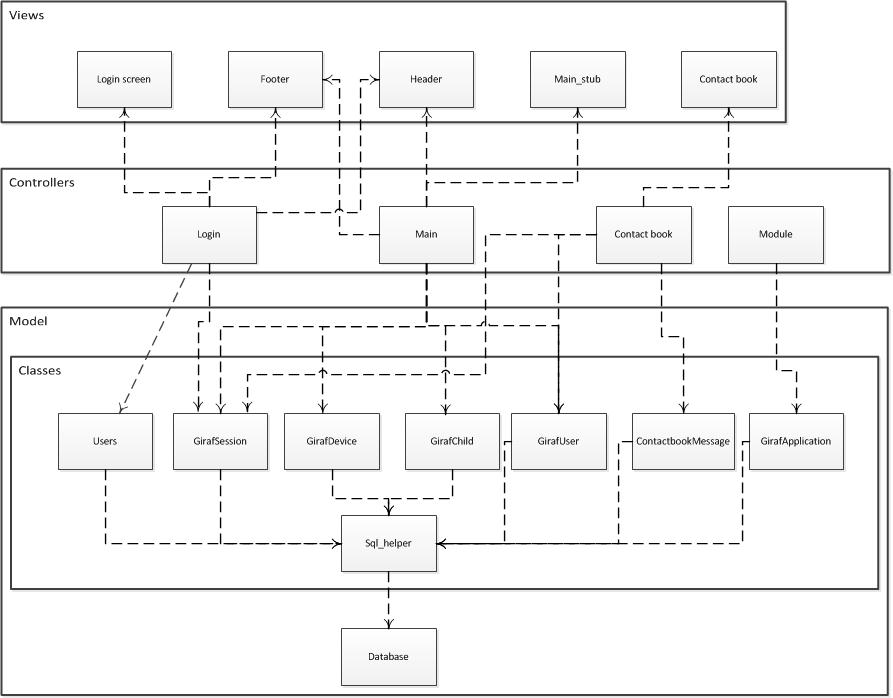
\includegraphics[width=1.00\textwidth]{img/overview.jpg}
	\caption{model-view-controller overview}
	\label{fig:overview}
\end{figure}

\section{Model}
\label{model}
This section describes how the model was implemented into GIRAFAdmin's MVC architecture. In particular implementing a combined Active Record/Factory pattern and automating the model's self-defining properties are described.

\subsection{The GirafRecord class}
\emph{GirafRecord} is designed as a combination of the Active Record and Factory patterns. Subclasses of G\emph{irafRecord} need only specify their source table and associations within overridden methods \emph{getSourceTable}, \emph{getPrimaryKey} and \emph{setAssociations}. Using this data, \emph{GirafRecord} determines the appropriate class to instantiate upon request through the \emph{getInstance} method (which is proxied automatically into methods in the format ``getClassName'' - for example \emph{getGirafChild} for the class \emph{GirafChild}) and dynamically creates the members necessary to properly represent the underlying database table. Thus changing the value of a field (member) for a row (object) is only a question of changing the value of that object's corresponding member (user $\rightarrow$ statusKey in the case of \emph{GirafUser}, for example). Changes are not written back to the database until \emph{commit} is called on the object.

The class diagram in appendix \ref{diagramAppendix} shows the relation between the \emph{GirafRecord} class and its subclasses.

\subsection{Dynamic shaping}
Thanks for the dynamic typing properties of PHP, object of classes can be modified during run-time. PHP also has several so-called ``magic methods'' that can increase the flexibility of classes. Three of these, two for properties and one for methods, was applied to dynamically shape objects to the tables they were representing.

\subsubsection*{Properties}
PHP defines the class methods \emph{\_\_get} and \emph{\_\_set}. They are called whenever a non-existing member is requested. For \emph{GirafRecord}, this means that although table columns are not defined as members in the class, they are available at run-time. \emph{\_\_get} and \emph{\_\_set} perform lookups in a private array of key-value pairs that match the table's structure, and registers any changes to the data.
Both row structure and data are returned as an associative array through PHP's MySQL functionality, and distilled into the internal data array where \emph{\_\_get} and \emph{\_\_set} and work with it.

\subsubsection*{Methods}
The methods \emph{\_\_call} and \emph{\_\_callStatic} are defined with similar usages as \emph{\_\_get} and \emph{\_\_set}, only with object and class methods, respectively. \emph{GirafRecord} overrides \emph{\_\_callStatic} to offer an instance-retrieval method that matches a subclass. This is merely a proxy for \emph{GirafRecord::getInstance}, but makes for slightly more readable code. For example, the class \emph{GirafUser} automatically defines \emph{getGirafUser}, \emph{GirafGroup} defines \emph{getGirafGroup} and so on.

\subsection{CRUD}
\emph{GirafRecord} only defines functionality for creating, reading and updating records in the current implementation. Due to the complications of retaining key integrity across table associations, row deletion was never implemented. Although the InnoDB engine (used in all the Giraf database tables) supports this integrity, relying on that implementation would rule out the use of any other database system or even MySQL engine, severely reducing the portability of the system.

\subsection*{Create}
Creating a new record simply involves creating a new instance of the desired record, settings its values and calling the commit method. Each \emph{GirafRecord} maintains a private array of which fields have been changed since initialisation. During creation of a new record only these values are set, any unset values are set to null.

\subsection*{Read}
Retrieving an existing record is achieved by calling the \emph{getInstance} method (or its subclass equivalent) and passing the primary key value of the desired row to it. If it exists, an object is prepared, ready for consumption and false (a typical PHP failure value for function calls) if the record does not exist.

\subsection*{Update}
Updating is performed first by reading an object, changing values (as with creation) and finally committing. Like the create flow, \emph{GirafRecord} registers changed fields and only updates them.

\subsection{The MySQL database}
Early on in the project, the previous group's GirafPlace database (responsible for registering GIRAF applications and making them available for download to devices) was merged with the new emerging GIRAFAdmin database in order to create a single, centralised system. It contains tables with data about administratiors, applications, children, groups, devices and more.
As described in subsection \vref{design_tech_model}, the \emph{GirafRecord} base class follows the Active Record architectural pattern. Thus, in order to retrieve rows from the table \emph{devices} the corresponding model class \emph{GirafDevice} is instantiated through the static \emph{getGirafDevice} method.

\subsubsection{Database relations}
MySQL supports a number of database engines, different implementations that offer varying levels of performance and added features. Among them, only one supports explicitly defining associations/relations between tables and only for the purposes of concurrency and bloat reduction. This necessitates a different approach to defining strong associations between tables. In the current implementation, it is achieved by using static methods overridden in each subclass of \emph{GirafRecord} or residing in the base class.
\emph{addAssociation} connects two \emph{GirafRecord} subclasses within the context of an association table - that is, a table that only contains a primary key (denoting a single relationship), a left (or parent) key to one half of the association and a right (or child) key to the other half. The designed associations can all be viewed in appendix \vref{fig:database_relations}.

As a convention (and solid design), every single table in the database contains a primary key that can be used to uniquely identify a row within the table. In general it is referred to as the table name in singular appended with ``Id'' (for example, the table \emph{devices} has the primary key in the field ``deviceId''. This is the key referenced either as a left or right part of an assocation. Note the convention of calling the value an ``id'' when referenced locally (within a single table) and as ``key'' when referenced remotely (also sometimes referred to as a foreign key).

Any one-to-one or one-to-many associations are implemented using only the two tables involved. In the case of users, for example, any one user can only have one active status (online, offline, away) at any given point. That status, however, may be applicable to several different users at once. Thus ``statusKey'' is defined in the users table to reference which status is currently active, while the status itself has no relation in the other direction. This also demonstrates why describing an association as a parent-child association (downwards) communicates the direction and nature of the association, while ``left-right'' is meant for uni-directional associations.

Many-to-many associations must be implemented with an extra table; the aforementioned association table. In the case of groups, for example, a group has a number of users attached to it. Conversely a user may be a member in any number of groups. Defining a new table field for each (possible) association causes unnecessary and indeterminable bloat (four association fields are unnecessary for a user in a single group, while it does not suffice for a user in eight). An alternative is to register all associations in a single field, delimited by a special character (commas, for example). This approach requires more logic to be implemented in the model and uses less of the power of relational database systems. Using association tables are the clear choice.
\section{View}
\label{view}
In this section we explain our thought on designing the visual part of GIRAFAdmin. We wanted to create a simple and pleasant design for the user and it was crucial that the design was intuitive to use, as the user may not be experienced with computers. \todo{Why are we discussing aesthetics in a technical chapter? - Joe}

\subsection{Technology}
As GIRAFAdmin is web-based, the most obvious choice for implementing viwes are through the de factor standards of (X)HTML and CSS. Apart from this, using JavaScript (notably with the JavaScript library JQuery) offers more reactive web pages that can be made to only reload partially instead of completely reloading the page on every new request. See chapter \vref{implementation_tools_languages} for an introduction to the various tools and concepts. Do note, however, that the specific divison between controller and view means that a controller action could as well invoke views that create a HTML5 web page as it could invoke a view that created and displayed a PDF file.

The following figure depicts the most predominant output of the current (HTML) implementation and the views and segments it is split into. Note in particular the header and footer of the page (much of it invisible to the user as it merely sets up the environment), which can be re-used in other views to create a global style and functionality to the site. The division is made from a conventional divide and conquer methodology. By solving the issue of CSS style and JavaScript inclusions in one place, they can easily be upgraded or switched out in one place while still affecting the entire site. Conversely, removing the redundancy from all "content" views (views with the actual content or representations of the model) makes for a cleaner base template for views and their interchangeability.
\missingfigure{Full-screen image of the main page with an open contactbook. Mark all special sections.}

The views in MVC represent everything that is displayed to the end user. There is some leeway in the pattern specification as to how the view is accessed. GIRAFAdmin follows a method used by several MVC frameworks where the view is invoked and displayed by the controllers after user input has been parsed and interpreted. Each view is a PHP script file. By this virtue there is no requirement that the output be HTML - a controller for listing users in the GIRAFAdmin database could as well output a full web page as it could output a PDF file generated by LaTeX or JSON data for cross-site API usage - the latter is actually an output format used to implement AJAX in the main view to deliver a more reactive user interface.

\subsection{Structure}
View files are placed in the \emph{/views} directory where they can be invoked by a controller using GirafController's view method. Views specific to GIRAF applications (such as Contactbook) should be placed in uniquely named subdirectories in the \emph{/apps} folder. Core views for GIRAFAdmin are placed in \emph{/default}.
As noted earlier, views are separated into three parts: header, footer and content. Implementing global header and footer views makes it a simple matter to quickly change the global style of the entire site or inject content into documents that already have defined header sections. In fact, although sub controllers like Contactbook are injected into the content view \emph{main\_stub}, this approach allows for the sub controllers to be displayed by themselves simply by prepending a header and appending a footer, resulting in a very flexible view structure.
Although views can, in principle, perform the same actions as controller and model (as there is no scope or script restrictions) it is highly discouraged. Instead, views should rely solely on the output functions of PHP and the variables initialized by the calling controller. When a view is invoked, it is passed (by value) a set of variables from the controller and is implemented to display or discard data as necessary for final output to the calling environment.

\subsection{Code}
Views have no governing base class like the model's GirafRecord or controller's GirafController. Instead, each view file should be specifically tailored within its domain and role. All currently implemented views, for example, are written within the header-content-footer style, outputting HTML for display in browsers.
Creating new views has to be done within the purview of new or existing controllers. A view cannot be displayed without a controller to supply relevant information from the model's current state. While not impossible, it is more likely that new views will be introduced to controllers than two different controllers will invoke the same view.

\subsection{Current views}
In its current iteration, GirafAdmin has six views. A single header (header.php), footer (footer.php) and four content views, login, main (main\_stub), Contactbook/list and Contactbook/show. While each content view expects the header to be loaded, they are completely independent otherwise. This means that although Contactbook is loaded inside of main\_stub, it can just as easily be displayed on its own.
\section{Controller}
\label{controller}
This section will discuss the controller layer of the \emph{GIRAF} site, in particular the \emph{GirafController} class as well as the interplay of JSON and the incomplete views that are output by certain controller actions. The discussion will center on the philosophy and inspirations behind the technical design of the controller, finally leading to the implementation that was completed as part of the this project period. The section will end with an overview and an example usage of the three base scenarios envisioned for \emph{GirafController}.

\subsection{Technology}
The method of input/output is highly inspired by several existing web-based MVC frameworks, most notably Ruby on Rails and CodeIgniter, as mentioned earlier - the specifics will be discussed in subsection \vref{controller_design}.

\subsection{Base concept}
Ensuring that the security concerns voiced by Birken (see appendices \vref{first_interview_birken} [47:40] and \vref{sec_interview_birken} [54:00]) would be addressed was a key factor when considering how to implement the input/output flow through the website.

\subsubsection*{Security concerns}
The assets that need to be secure are universally defined as the user-generated content associated with users and children. In the specific context of this project, this is their personal details, contact book messages and the attached images. There are two steps to securing the data. First of all, data should be stored in a database with strict access rules. In MySQL it is possible to restrict access to the GIRAF database down to a single user and source address. Specifying that only the local system may access the database effectively eliminates direct intrusion into that part of the system. However, images and binary data in general are a point of contention in regards to storage. Some argue, that it improves security and reduces overhead on file systems, others take the point, that storing and retrieving large blobs of data risks locking up the database for further requests, while transfers are in progress. Three approaches to securing such data are described as follows:

\begin{description}
    \item[Temporary files] One approach involves copying inaccessible files to accessible locations on the web server with randomly generated names. Once the images have been loaded by the client they can be safely removed (images are transferred during page load and not used for the remainder of the page display). Disk usage can further be reduced by using linking features specific to operating systems (Linux systems' ``ln'' command or Windows' junction points), eliminating redundant versions of identical files. This approach presents the same basic vulnerabilities as the current implementation (files are externally accessible), but to a much lesser degree (only files currently in use are exposed). However, this comes at the cost of file maintenance. Server-side scripts will need to remove the files when they are no longer required.
    \item[Direct image output] Another approach is to store files in a location that is inaccessible to external sources, and output the content of the files through the MVC framework directly to the client. The difference between transmitting a page of HTML or binary image data is discernible only by the actual data and the \emph{MIME} (Multipurpose Internet Mail Extensions)\cite{MIME} type reported by the server during transmission. Using this approach will make it possible to access all resources through a single access point (for example, a controller that receives resource identifiers and outputs their contents if the request can be authorised), giving strict control over access. An added benefit is that the actual resource data can be stored in any location that is reachable by the server-side PHP code, be it file system, within databases or on remote servers. The only immediate downside is the added overhead of the script that needs to output the data (in contrast to regular file accessibility, in which only the web server is active in delivering data).
    \item[Authentication schemes] A third approach is to use one of the many authentication protocols supported by HTTP to restrict access to externally accessible resources. While this vastly simplifies the storage of resources on the server (to the level of the current implementation), it bears the need to implement support for the authentication protocol in the web pages and may require additional software on server or client.
\end{description}

Each approach has merit depending on the context, although the final level of security increases roughly from the first approach to the last. The second approach is both simple to implement (all of the required functionality exists in PHP) and exhibits a level of access control that is only limited by the robustness of the code. There are still types of attack that the code is vulnerable to:

\paragraph*{Injection attacks}
Injection attacks involve a malicious user sending unexpected input values. Typically they will anticipate an SQL selection query in the style of ``SELECT data FROM table WHERE username='some\_name''', where \emph{some\_name} is replaced with the user's input. If the input is not properly sanitised, a malicious user could send an input like "' OR TRUE=TRUE" OR '". Pay close attention to the additional quotes that will effectively end one SQL condition, add a tautology and properly end the condition, resulting in "username='' OR TRUE=TRUE OR ''". The user has \emph{injected} new executable code into the query, an unintentional and dangerous security hole. The solution is simple to implement, though difficult to perform comprehensively. Any input strings from the user should be sanitised (made safe) by escaping (prepending backslashes to) any characters that bear special meaning in SQL contexts. Quotes in particular, should be escaped to avoid execution to run outside its intended area.

The seeds of the resource access restrictions already exist in the framework. The site is intended to be used by clients exclusively through the execution of the base index.php script as well as access to two key directories: CSS (for stylesheets) and JS (for JavaScript files) - neither contain confidential information, only resources necessary for proper rendition of web pages. A default web server configuration will typically allow access to all resources, requiring additional setup when installing the software on a new server. See the appendix \vref{appendix_server_conf} for an example configuration used by the project group's installation. It restricts access to all other resources than the one file and two directories named, redirecting all unrecognized requests directly to the index.php file. This adds the benefit of making a cleaner, more easily read \emph{URL} format (http://www.giraf.dk/contactbook/list/3 as opposed to http://www.giraf.dk/contactbook.php?action=list\&userid=3).

\subsubsection*{File structure}
All controllers reside in the \emph{/controllers} subdirectory of the web site document root. Furthermore, given the convention of placing GIRAF application-specific data in \emph{/apps} subdirectories, any administration controllers offered by uploaded GIRAF applications are stored in such a directory.

It is the intention that all controllers callable directly by the user reside in that root, while all GIRAF application controllers (referenced as \emph{sub-controllers}) must be accessed by primary controllers. A special controller for this purpose (the \emph{Module} controller) exists to allow restricted access to them externally - this is more a user-friendly filtration than a security measure. \emph{Module} has the capability to ensure that the child/device/app configuration requested is valid, reducing the risk of corrupted or bad page reads.

\subsection{Controller design}
\label{controller_design}
As mentioned the GIRAF MVC design is highly inspired by that of other web-based MVC frameworks, in which each controller is represented by a subclass of a base controller class. Barring a few special name cases, each public method of the class is considered an action that can be invoked directly by a client.
In the case of the GIRAF site, the base class is \emph{GirafController} (an abstract class) and the only two special methods are \emph{index} and \emph{fallback}. \emph{index} is used as a default action if the controller is invoked without any specific request. \emph{fallback} is used when an unknown action (non-existing method) is requested.
Finally, \emph{GirafController} implements a method, called \emph{view}, that parses a single view file from the document root's \emph{/views} folder. \emph{view} optionally takes an associative array of values to be made available to the called view. This is done by extracting the values and storing them in variables with the same name as that value's key. The value 14 in the array index ``userId'' would thus be available in the view as the variable ``userId''.

\subsection{Implementation}
As the primary access point to GIRAFAdmin for users, controllers are exposed simply by accessing the web server with an appropriate URL. With a proper server setup as described earlier, all unrecognised server requests go through index.php. The file performs the following actions in order before any output is sent to the client browser (in fact, all output is suppressed from the URL parsing until controller invocation has been resolved):
\begin{enumerate}
    \item \textbf{Authorisation} If no user has been logged in (that is, if no active PHP session can be found), the user is forced into the Login controller if it was not specifically requested. This makes it impossible to access the rest of the GIRAFAdmin site without being registered and authorised.
    \item \textbf{URL parsing} The requested URL (for example ``/login/register'') is parsed into an array of parameters more easily digested by later code. The first element after the document root is put into the index ``controller'', the second into the index ``action'' and all following elements in ``paramX'' indices, where \textbf{X} is the zero-based number of the parameter.
    \item \textbf{Controller invocation} Assuming a controller was requested (if not, \emph{Main} is set as a default), the subdirectory \emph{/controllers} is searched for a file with the same name as the requested controller (in a case-insensitive manner). If it is found, that single found is included into variable scope. If not, all files in the directory are included into variable scope and all newly-defined classes are searched (this is a more resource-demanding process and therefore used only as a last effort). A new object of the class is finally created, or if the controller was not found an error is thrown.
    \item \textbf{Action is called} If no action was defined, the controller's index method is invoked. Otherwise, the controller object is polled for the requested action. If it exists, the corresponding method is invoked with the URL path (now in array form) as parameter. If not, the fallback method is invoked instead.
    \item \textbf{Invocation returns control} The controller passes control back to the main thread and the output buffer is flushed, finally sending output to the browser.
\end{enumerate}

\subsection{Usage examples}
This section briefly describes the three primary envisioned usage scenarios of \emph{GirafController}: a core controller, a minimal-output controller and a GIRAF application sub controller.

\subsubsection*{A normal controller}
The controller \emph{Main} makes use of all of the base functionality of \emph{GirafController} and thus proves a solid example of core usage.

\lstinputlisting[language=PHP]{tex/implementation/controller_example_main.php}

Notice how the controller \textbf{always} defers control to \emph{fallback} that ignores any extra parameters and simply shows the default page. A complete page for display is typically comprised of a header (that contains starting tags for HTML and body tags, HTML doctype and any global JavaScript and CSS file links), a footer (that closes tags from the header and may contain global footer content) and main content. Note in the code that three views are loaded by \emph{Main}: header.php, main\_stub.php and footer.php. Both header and footer are also used by the controller \emph{Login} and should be used by any \emph{GirafController} that displays a full page to the user (future examples could include account, user and group administration pages).

\subsubsection*{A JSON controller}
\lstinputlisting[language=PHP]{tex/implementation/controller_example_child.php}

The controller \emph{Child} demonstrates how an already generated web page can request new data in the background in order to reduce page loads, but also introduce a more dynamic page impression. In its current implementation this kind of controller exclusively outputs JSON-encoded data that can be readily consumed by the JavaScript already loaded by the client. It is debatable whether the direct output of JSON-encoded data from the controller (and not an actual view) goes against the MVC pattern.
The JSON controller type is not a subclass in itself (yet), but is intended to pass simple data structures back to the client, enabling both AJAX from the browser but also enables an external API that can be utilized by other sites for greater utility of the framework
\newline
\subsubsection*{A sub controller}
\label{controller_sub}
\lstinputlisting[language=PHP]{tex/implementation/controller_example_contactbook.php}

The controller \emph{Contactbook} is currently the only example of a sub controller and is thus partly intended as a practical example of how new GIRAF-compliant applications can offer customised administrative functions for users beyond a simple control over the settings of the application on a device.
Of greatest interest (and the feature that most notably makes the controller a ``sub'' type) is the lack of header and footer views, or their equivalents. These controllers are designed to be injected into HTML that is already loaded with the necessary data to run in a browser. Thanks to the flexibility of the DOM it is possible to add stylesheet and javascript files after the document was originally loaded, in principle making it possible to traverse the entire GIRAF site without ever replacing the header and footer sections.
Of smaller note is the action  \emph{\_list}. In PHP the word ``list'' is reserved and cannot be used for any definitions. However, the name was a prime candidate for the name of an action. A workaround is to utilise \emph{fallback} to check if the requested action is ``list''. If it is, execution is passed to \emph{\_list} instead.
\newline
\subsection{Implemented controllers}
Following is a quick list of the controllers currently implemented in GIRAFAdmin. They are divided into the aforementioned three groups: main, sub and JSON controllers.

\subsubsection*{Main}
GIRAFAdmin has two main controllers in the current version for direct user interaction, \emph{Main} and \emph{Login}, as well as a single controller meant for sub controller interaction - \emph{Module}.
\begin{description}
    \item[Login] is for user authentication, registration and aid in case the user has forgotten their password.
    \item[Main] is used as a primary overlay and access point to administration of all children, devices and applications.
    \item[Module] is used as a proxy for all controllers associated with applications that need to be managed through GIRAFAdmin. Requests are passed almost transparently through to the requested sub controller, but basic authentication measures can ensure that unauthourised access is halted.
\end{description}

\subsubsection*{Sub}
As mentioned in subsection \vref{controller_sub}, only one sub controller is currently implemented - \emph{Contactbook}. It exposes all the functionality that a user should directly be able to access as defined in the original design (message listing, creation, replies and such).

\subsubsection*{JSON}
The GIRAFAdmin view \emph{main\_stub} makes significant use of AJAX to request new data after a page has loaded. In order to simplify request of the data, and reduce bandwidth usage and processing requirements, only the most necessary data is transferred. The current four JSON controllers (\emph{App}, \emph{Child}, \emph{Device} and \emph{Group}) are all variants of a basic data retrieval mechanism - their names directly reflect what type of information they output. \emph{App} outputs information about installed applications, \emph{Child} about children, and so on. They can list data associated with a single entity (children to a user or apps on a device, for example) and return it as a JSON-encoded string that can be consumed by JavaScript.

\section{Conclusion}
In conclusion, the current implementation of GIRAFAdmin has an open and flexible approach to the MVC pattern. The way page requests are parsed into parameters makes implementing new controllers a simple task of creating a new subclass in the correct directory. Furthermore, several methods offers simple ways of controlling default behavior, unexpected input and view loading.


\chapter{Summary}
%Hvad fik vi med i programmet. MVC struktur, working contact book 
%Opsummering p� hvad vi har skrevet i delen Implementationen.

The final version at deadline contains an extendable framework, supporting both extension of the core system and adding functionality for new GIRAF applications by plugging in new MVC components.
The core system contains basic access control, database abstractions through the model layer and an MVC API that should simplify future development.
As a proof-of-concept in the implementation, a working contact book is implemented.

%Seriously guys, I have no clue what to add....
%I've read the implementation part 3 times now and still nothing....


% 4 System evaluation
\part{System evalution}

\chapter{Unit Testing}
%unittheory og unittest
\section{Unit test theory}
% Form�l med unittest, hvad kan unit test bruges til 
% basal termenoligy, der findes test opensource => simple test  
A unit test is a testing method that can be used to asses if already written code works as intended. In the unit test case has been made an assumptions and if the assumption turns out to be wrong then the code has failed. The developer will fix the bug and try again until the assumption is true that means the unit test passes. A unit test should only test particular method or function within the tested code. (kilde: The Art of Unit Testing: with Examples in .NET, Roy Osherove, Manning Publications, 2009)
To make a good unit test this should be followed: according to Roy Osherove\cite{AOUT}: 
\begin{itemize}
	\item It should be automated and repeatable
	\item It should be easy to implement
	\item Once it's written, it should remain for future use
	\item Anyone should be able to run it
	\item It should run at the push of a button
	\item It should run quickly
\end{itemize}

\subsection{Reasons for using unit test}
When a unit test is performed it is because the developer wants to know if his/hers code run as it is supports to.  An advantage of unit testing is that the test can run separately from application such that parts of the application can be tested in isolation\cite{UTF}. Another advantage is that the developer can test several test cases together or one-by-one and later in the development process the developer can still use the test.  

This test can only be used to determine if the code is good and working, and if the test suite of unit test has a high code coverage and many assertion then it is an indication of that the code is of good quality. Other test are necessary to test e.g. the application usability.   

\subsection{Unit test frameworks}
The advantage for using a unit test framework is that the developer does not have to program it, which would be very time-consuming. Unit test framework help the developer to write a test more quickly and it can run the test and review the result more easily\cite{UTF}.  

There has been made many open source unit test framework for various coding languages and development platforms. These frameworks are generally known as xUnit. E.g. is  CppUnit for C++, JUnit for Java, NUnit for .NET among the xUnits\cite{UTF} and for PHP coding language is SimpleTest also a unit testing framework.

\subsection{}
Before writing the test the developer has an assumption of how the code behaves for a given input and then expects a certain output and this is assumption is validated in the unit test. A unit test consists of three parts\cite{AOUT}: 
\begin{itemize}
	\item Arrange
	\item Act
	\item Assert
\end{itemize}

In Arrange objects is created and made ready before Act which calls the code that is being tested and thereafter in Assert the premade assumptions about the return value of the tested code is validated. A unit test framework contains assert classes that have several methods the developer can use to verify the code.  E.g. it can check if the output is null or if an exception has been thrown.


\section{Unit testing process}
In our unit test we have used the php unit test framework SimpleTest, which meant that we only had to write the unit test cases and the specified test suite. First where will be listed what was tested and then a few examples will be shown. 

\subsection{Test cases}
% afd�kke hvad der kan testes med denne test,
% lav en liste over hvilke dele der bliver testet
This unit test was made to test some of the classes in the model layer performed as expected. Each test case tests only one class from the model, but the test case contains a test for each function there are in the tested code. The class AllTests is our Test suite and the test cases is listed below with its test functions:

\begin{itemize}
	\item {\textit{TestGirafNewsPost} tests the class \textit{GirafNewsPost}}
		\begin{itemize}
			\item {\textit{testBaseGroupNews} tests the function \textit{getGroupNews()}}
			\item {\textit{testSingleGroupNews} tests the function \textit{getGroupNews(1)}}
			\item {\textit{testUserNews} tests the function \textit{getUserNews()}}
		\end{itemize}

	\item {\textit{TestGirafGroup} tests the class \textit{GirafGroup}}
		\begin{itemize}
			\item {\textit{testGetFunction} tests the function \textit{getGirafGroup(1)}}
		\end{itemize}

	\item {\textit{TestSqlHelper} tests the class \textit{sql\_helper}}
		\begin{itemize}
			\item {\textit{testInitialization} tests the function \textit{getConnection()}}
			\item {\textit{testGoodQuery} tests the function \textit{selectQuery()} with valid input}
			\item {\textit{testBadQuery} tests the function \textit{selectQuery()} with invalid input}
		\end{itemize}

	\item {\textit{TestGirafUser} tests the class \textit{GirafUser}}
		\begin{itemize}
			\item {\textit{testGetFunction} tests the function \textit{getGirafUser(1)}}
			\item {\textit{testOnlineStatus} tests the function \textit{getOnlineStatus()}}
			\item {\textit{testGetGroups} tests the function \textit{getUserGroups()}}
		\end{itemize}

	\item {\textit{TestAuthFunctions} tests the \textit{class auth}}
		\begin{itemize}
			\item {\textit{testHash} tests the function \textit{hashString()}}
			\item {\textit{testPasswordGet} tests the function \textit{auth::getPassword(1)}}
			\item {\textit{testPasswordMatch} tests the function \textit{matchPassword()}}
		\end{itemize}

	\item {\textit{TestGirafChild} tests the class \textit{GirafChild}}
		\begin{itemize}
			\item {\textit{testGetFunction} tests the function \textit{getGirafChild(1)}}
		\end{itemize}
	 
\end{itemize}


\subsection{Implementing the test}
\todo{tester en klasse pr fil, man kan teste en eller alle filer.
 et kode fra unittest, test_full + en testcase.}


\subsubsection*{Test suite AllTests}
\lstinputlisting[language=PHP]{tex/evaluation/test_full_example_testSuite.php}
\todo{kommentar til AllTests}


\subsubsection*{Test case TestGirafUser}
\lstinputlisting[language=PHP]{tex/evaluation/TestGirafChild_example_testCase.php}
\todo{kommentar til TestGirafUser}

\subsubsection*{Conclusion}
\todo{alt fungere p� nuv�rende tidspunkt}


\chapter{Usability Testing}
% indeholder usability.tex og usabilitytest.tex
After designing and implementing the contact book, the system was usability tested by Kristine Niss-Henriksen. This was done in the third and last interview with Kristine.
This chapter contains some theory about usability and a description of the usability testing process.

%After the implementation of the contact book the system was tested and this chapter include theory of usability and the result from a usability test, that performed by Kristine Niss-Henriksen in the third interview.
  
\chapter{Theory}

\section{Usability}
When developing software and other products that require user interaction, one must be aware of the usability of the product and how to evaluate it.
Usability is a quality attribute, which is fundamental to a successful product and is defined by 5 quality components:
\begin{itemize}
	\item Learning: How easy is it for users to accomplish tasks during first encounter of the design. 
	\item Efficiency: After learning how the product works, how fast can they perform various tasks.
	\item Memorability: After a period of not using a product, how easily can they obtain efficiency again.
	\item Errors: How many errors do users make and how easily can they recover from the errors.
	\item Satisfaction: How pleasant is it to use the product.
\end{itemize}

To explain the importance of usability and how it is fundamental to a successful product, one must understand that no matter how a product functions, as long as user interaction is required, it must comply with the needs of the user and help to complete the tasks at hand.
As an example one can look at a website. If a website is difficult to use, if users get lost trying to browse the website or the information stored on the website is hard to read and/or figure out, people tend to look for alternatives. This results in loss of customers and therefore is bad for the company that designs, hosts and administrates the website.
If a product on the other hand is designed for a special purpose where no alternatives are to be found, like a system to administrate a hospital. Usability is so important that errors could lead to serious harm of patients. Reasons can be efficiency or errors, where time spent figuring out the system means delay in service and errors can result in system stalling or misinformation.

There are methods for studying and improving usability but user testing has proven the most useful and will therefore be the project�s focus when evaluating usability of the product.\cite{usability}
\section{Usability testing process}
To receive feedback on our prototype, we decided to conduct a usability test. Our testing subject would be an actual user, in this case the kindergarten teacher Kristine Niss-Henriksen.
\subsection{Planning}
% write out testing times (the third meeting) and note what we wanted to test (which features?) and which attributes of those features we'd like to determine the usability of (for example, ease of use, if enough of the features are supported, etc). 

In our usability test we wanted feedback on a number of areas; one being the general layout, such as the double menu, creating a combination of the two axes. We wanted to test the intuition of the menu, as it is one the core parts of the prototype. 
 
Furthermore we wanted to receive feedback on our contact book, which has been a focus point in our prototype. The prototype should provide a simple overview for the user. To test this, we instructed our subject to carry out simple tasks to see how the user reacted.


\subsection{Third meeting \& testing}
% already in process, this was very informel remember to note that.

During the interview (see appendix \vref{third_interview}) we showed the prototype to our subject. She was first presented with a login screen, where the subject was instructed to create a new user. After a login was created, the subject proceeded to login and was directed to the main window. We gave a brief introduction to the layout and proceeded to guide our subject through further tasks, such as creating a new post in the contact book, adding images to a post and reading existing posts. 


\subsection{Evaluation}
% what did we learn from the meeting. 
Our first attempt to run the prototype failed as our subject used an older browser on her computer, which is an unavoidable problem and should be fixed.

When our subject was first introduced to the login screen, she created a new user and logged in without trouble. However we noted that she expected the mouse to automatically focus on the input field, after she typed her information incorrectly. Furthermore it was not possible to use the Enter-key to submit user credentials. This should be easy to patch.

When our subject was presented with the main window, she immediately turned to the menu for the next step. Although the menu was buggy, we managed to pull through. As our subject was asked to create a new post in the contact book she mistook the headline submit box for the body text, which means, the layout should be different. 
Furthermore, we received feedback on how the contact book should work, i.e. how and when a post is marked as ``new'' or ``unread''. We presented an idea in which a new post would lose its status as ``new'' if simply one colleague opened the post. This could improve efficiency as the individual could read a post on behalf of the kindergarten. However the kindergarten teachers at the kindergarten would read every mail regardless of content, the idea of sharing ``New post'' with colleagues was abandoned. 
Additionally she emphasized the idea of having a print function, which would print posts from a child's contact book, as this often plays a major role in the child's life. This function should be easy to access for the user.




\chapter{Conclusion}

% 5 Conclusion
\part{Conclusion}

\chapter{Further development}

In this chapter we express our ideas for further development, in contrast to what has been designed and implemented.

%er under chapter future work som 1. section
\section{Further development}

\subsection{Android}
We did not make an application for the child such that he/she would be able to see the images and image text from the contact book, which was one of the important functionality of the contact book.
%Christoffer

However, the designs for the protocol, client and server have been documented; implementing the features in protocol milestone 1.0 would make it a lot easier to develop an Android viewing application for the contact book, since it contains the basic functionality needed to synchronize and fetch data. In general; the next step would be to implement those features would be the next step. 
%Evt. skal Milestone 1.0 indsættes her - kommer når jeg lige har fået den på papir. Christoffer.  
%FUU too many steps ! (read rest of last sentence in Android). Birgir

\subsection{myAccount and News}
\label{myAccount}
%Maybe it should say somthing like: MyAccount and the News homepage was designed but not complitily implented - Ren� rettet:lisbeth
MyAccount and the News homepage was designed but not completely implemented. The model for both my account and News is done, but both controller and view is missing.

As in our design the myAccount would contain personal information and the user would be able connect a child to him/herself and connect the child with an device. Furthermore all the user's connected children would be able to be made into groups by the user.

In news a parent should be able to receive general news from the Kindergarten, while the kindergarten teachers also can add news.  

\subsection{Application administration}
We did not get to making an application administration system to aSchedule or DigiPECS. These administrations system would need the android synchronization such that the mobile devices' will be updated. 

The aSchedule administration would be like a normal calendar that also uses PECS to illustrate the child's schedule for a day. 

DigiPECS administration would be a program where the user could use to make and edit PECS, and it should then have access to an public archive of PECS (evt. opensource where the user also can add PECS) and a private archive for private pictures and PECS. 

\subsubsection*{Personalize}
This section should describe the "Settings" application, in which the user can edit information about the child and add/remove eventual handicaps. (It should also not be called "Settings" as it is an insensitive name.


\subsection{Site Admin}
Administering applications, groups and children are only the outermost pieces of the full scope of site administration. Tools for super users such as user administration and managing global application access (e.g. auditing and authorising new controllers for recently-added Giraf-compliant applications) should be staples.

\subsection{Delevoper guide}
During development of the first architecture it became evident that expanding the system was quite difficult, even with comprehensive code documentation. Writing a developer guide that describes philosophies, conventions and inspirations would be the next step in opening up the system to new functionality.

\subsection{Remote installation}
At one point it was considered that applications could be installed remotely, that is without a user installing from the device, instead marking applications for installation through the web site and the device performing the install on its next synchronisation.

\chapter{Reflection}
%indehoder:currentfunctionality, architecture, security, expandproblem, developmentmethod
In this chapter we reflect on the functionality and the architectural design of the implemented system.
Furthermore, we reflect on security concerns and how the current problem domain could be expanded without much adjusting.
In the end we take a look at our development methods, assessing the pros and cons of each.
Reflecting on these domains helps us to better realise the system and the development process.


%\todo{beskriver form�let med afsnittet.Hvad er det I vil reflektere over? Hvorfor reflektere overlige netop dette? Hvad kan I f� ud af det?}
\section{Current functionality}
\todo{vi er kun n�et et minimum. vi har en kontaktbog og login, men vi kan ikke tilf�je b�rn/device(MyAccount).
 en henvisning til futherdevelopment med hensyn til det der ikke er med. }
\section{Architecture}
%with this MVC is it easy to add more/new applications support
reflection on MVC
reflection on how implementations of new application administrator (as an aScheule administrator) in the giraf administration would be.
\section{Security}
\todo{"det sikkerhed vi har er segmentering s� user kun kan administratere b�rnene's mobile device. 
MVC opbygning g�r det umuligt at tilg� dele andet end controlleren.
Vi har ikke kigget p� kode sikkerhed, 
Billederne er frit tilg�ngelig, men man skal kende stien hen til billedet, dette skal forbedres, henvisning til Kristine 1. eller 2.
Password hashing
Hvis du log'er ind, tilg� alle handlinger p� controller, s� man kan tilg� andres b�rns devices. 
Stadig lidt s�rbart for indjection angreb"}
% under chapter reflection som 5. section
\section{Expanding the problem domain}
During this project we have based the product upon the needs of a kindergarten that has children with autism, however, the GIRAF-A-11 could be used by both children and adults with different disabilities and therefore the GIRAF-W-11 could be used by other institutions' employees, that works with these individuals or family members to the person with the disability. The contact book application could be used in its current functionality in schools, but it could adapted to become more like a diary for the adults with an disability.     

The GIRAF concept could be expand further to support individuals having problems using a mobile device. An example of this would be the elderly population that is uncomfortable using a modern mobile device because of the extensive functionalities and it small buttons. To accommodate these users a safe environment with different levels of restrictions could be made such that administrator of the device(the GIRAF-W-11 user) and the user would be able to sort in which application the user wants to have.\todo{Er det her stadig inden for vores concept? -lisbeth}

The GIRAF concept could also be used for younger children without any disability, where GIRAF Administration and the use of a contact book then also could enhance communications between parent and kindergarten or school teacher. Furthermore the GIRAF-W-11 then could include an application that forwards the child's homework to both the child and the parents, which also get solutions such that the parents are able to help the child with the homework. 

If the framework reaches a stable release (Android synchronization client, synchronization server and the possibility to manage groups) any organization or group in need of a closed application distribution and management form could use code to some extent - taking this a step further could be to extending the GIRAF platform to include and manage any type of application. 

    
\section{Development methodology}

\chapter{Conclusion}
In this report we primarily explain the development process of a contact book, created for employees of kindergartens working with children who has special needs and for the children's parents as well. The process contains interviews from where we received user feedback from a representative for these employees.

The contact book was implemented with all the earliest defined functionality - however, certain advanced features defined later were left unfinished. The contact book was implemented as a module of a web based application, the purpose of which is administering GIRAF applications and their settings. Because of limited development time and resources, the group focused primarily on the functionality of the product and less on security. Despite the group�s focus, the aspect of security is important, because the application handles sensitive personal information, on both the client- and server-side. A few basic security measures were implemented; some basic security holes were closed during development, however, several key types were left in the concept stage.

The web system, in it�s current state, is ready for further first- and third-party development through a documented framework that was designed and partially tested. While developing the system, a protocol for accessing information on a GIRAF mobile device was also developed, but not implemented.

To summarize, we have a working version of the contact book which meets the requirements of our usability feedback and testing. We have designed a framework to help future developers integrate their software into the existing system and a protocol which makes communication with the GIRAF mobile device easier. After analysis within related domains, developing and testing, we can conclude that our solution meets its basic requirements; basic functionality of the contact book is available and the web administration framework is partly implemented.


\addcontentsline{toc}{part}{Listings}
\listoffigures
\lstlistoflistings
\listoftodos
\label{lastpage}

% Change headings for bibliography. Looks fucked otherwise, I think.
% Page design from fancyhdr.
\fancyhead{}
\fancyfoot{}
\fancyhead[RO,LE]{\leftmark}
\fancyfoot[C]{\thepage}
\setlength{\headheight}{23pt}

% Afslut med bibliografien

\cleardoublepage
\phantomsection
\addcontentsline{toc}{part}{Bibliography}
\bibliography{bib/bibliografi}

% 4. Bilag
\appendix{}
\addcontentsline{toc}{part}{Appendix}
\chapter{Class diagram}
\label{diagramAppendix}

\begin{figure}[ht]
\centering
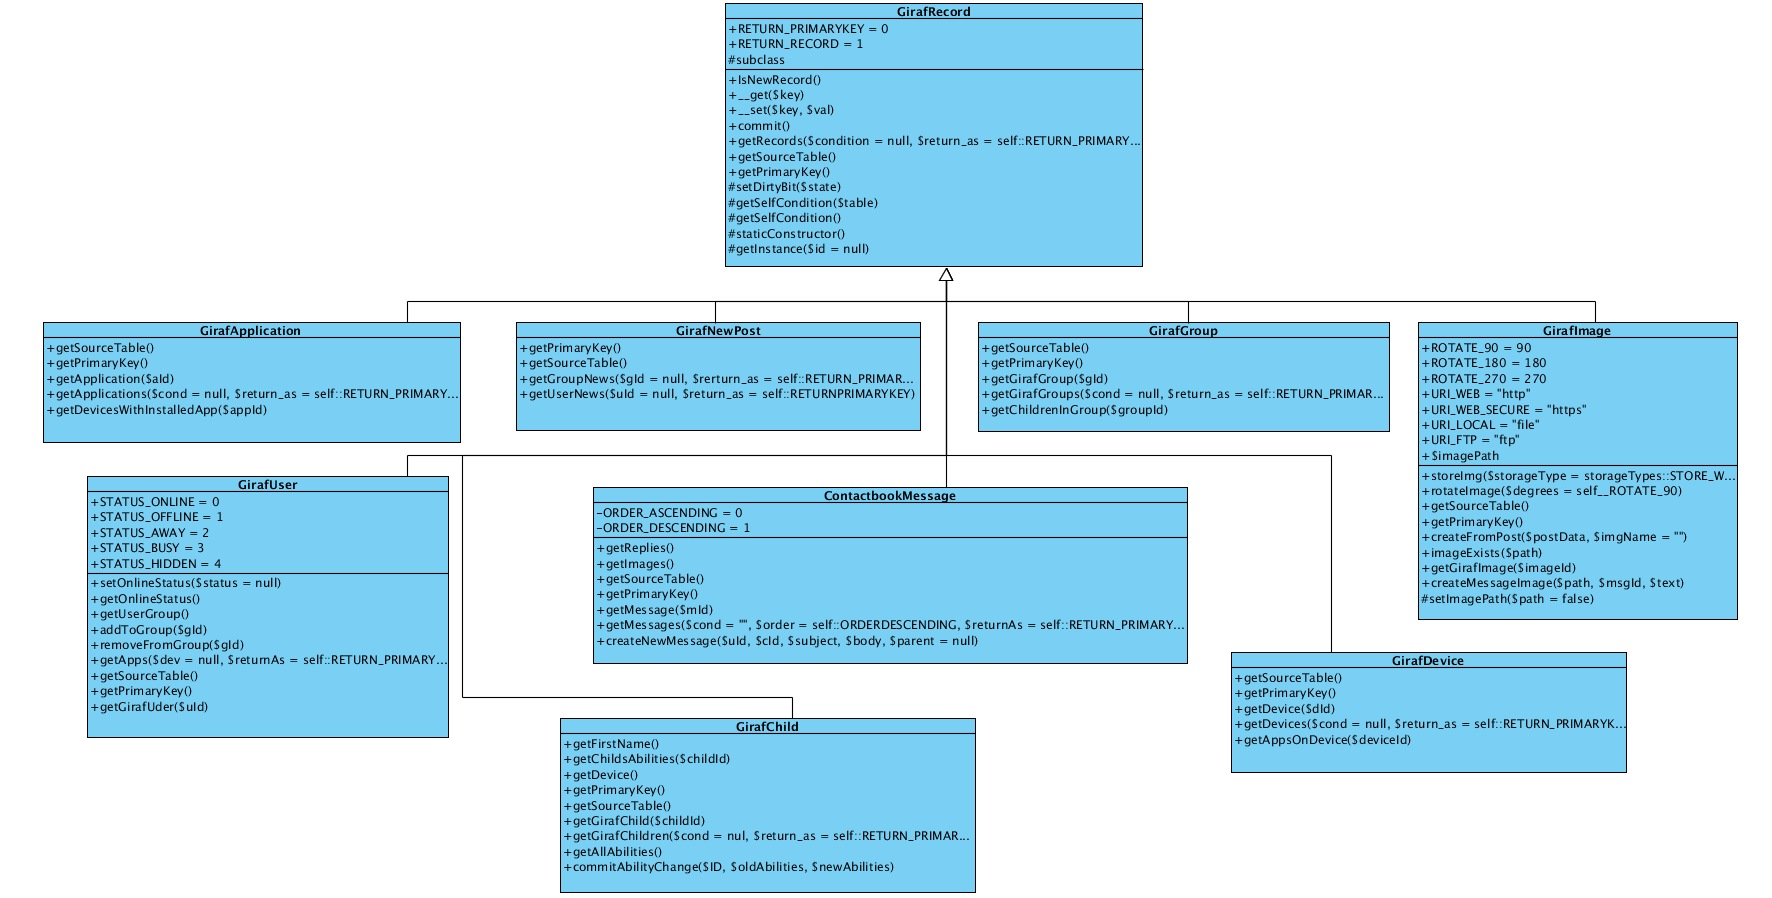
\includegraphics[angle=90,width=300px]{img/classdiagram_Fixed.jpg}
\caption{The figure shows the class diagram of the GirafRecord class, and its subclasses}
\label{fig:diagram}
\end{figure}

\begin{figure}[ht]
\centering
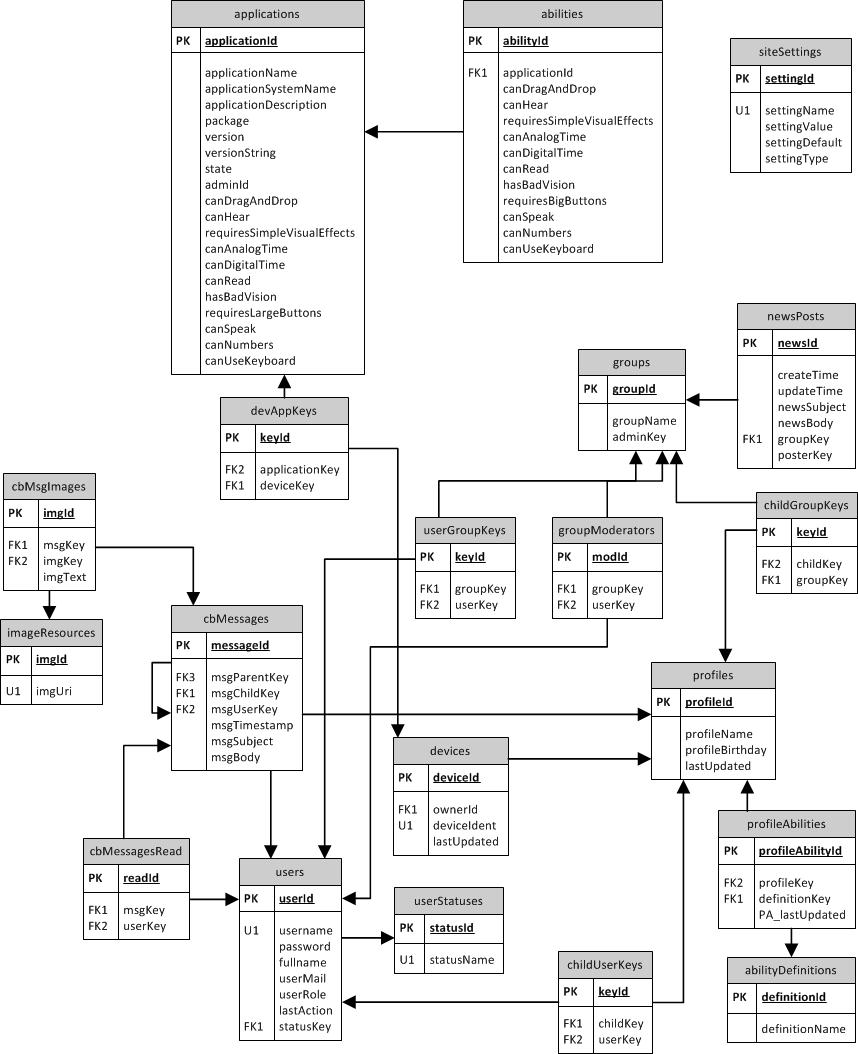
\includegraphics[angle=0,width=300px]{img/ER-relation(1).jpg}
\caption{The figure shows the relations between the tables in the database}
\label{fig:database_relations}
\end{figure}
\chapter{Interviews}
\section{First meeting with Birken}
\subsection{Disposition}
\begin{itemize}
	\item Avoid boolean or leading questions.
	\item Scenarios:
		\begin{itemize}
			\item digiPECS
			\item aSchedule
			\item plAytime (displays play instructions)
		\end{itemize}
	\item How could you administrate devices/applications? Suggestions?
	\item Rich pictures/images
	\item How do you create new or better meanings in communication?
	\item Prototypes
	\item Clear usage of time.
		\begin{itemize}
			\item Right now, what do the parents do, what do you do? (Explorative)
			\item Do you regularly discuss the child and their activities? How do you communicate? (Verification)
			\item Do you make detailed scheduling? Are the children involved in this activity? (Verification)
			\item How does a usual day play out? (Explorative)
			\item How do you communicate with the children? (Explorative)
			\item Reaction on removing their items (like a phone)? (Verification)
		\end{itemize}
\end{itemize}
\subsection{Questions proper}
\begin{description}
	\item[10 mins] Introduction (names, the group, overall project goals, our intentions with the meetings)
	\item[10 mins] Introduction of the currently working GIRAF system, excluding the admin app - this is done specifically to avoid associations with that app when IT options are discussed.
	\item[5 min] Our specific goal, a PC-based administration program.
	\item[20 min] How is a typical day (or week) structured for the supervisors?
		\begin{itemize}
			\item Areas of responsibility (parents vs. supervisors)
			\item How is planning done? During the work day and how far ahead?
			\item Does the institution have access to a PC?
			\item Variation in daily activities.
			\item Is it a realistic goal to give children access to a tablet? In an estimate, how large a group of the children are functioning high enough to work with such a device?
		\end{itemize}
	\item[20 min] Communication
		\begin{itemize}
			\item Which methods of communication exist for children with autism beyond imagery/pictograms?
			\item How is a single day's schedule presented? One event at a time or a large presentation at the beginning?
			\item How are new meanings introduced to non-verbal children? For example new pictograms.
			\item Are the children involved in deciding the activities?
			\item What kind of reactions could be expected from removing an item they consider theirs?
		\end{itemize}
	\item[25 min] abstraction to IT solutions
		\begin{itemize}
			\item Debate possible IT solutiosn to ease/improve the daily work.
			\item How can It improve your working day?
			\item Optionally consider directly discussing administration solutions or work with rich pictures. Bring blank paper to draw on if possible.
		\end{itemize}
\end{description}
\section{First interview with Birken}


Even before our input there was a clear desire to utilise IT to extend and improve communication by words.

Birken has a single child capable of working with actual words, otherwise the children most effectively communicate using the imagery of pectograms. However, the sounds, names and textual representations are very important in the discourse with guardians. Although a child may only signal a meaning with the image, they respond very strongly (and positively) to a reaction from the guardian if they respond with the word and possibly a complete sentence. While the child cannot speak the word, they can recognize it and the agreement in meaning is essential.

A flexible approach to imagery is very important. Images that most people would immediately understand with an exact meaning can be much more difficult for an autistic child to put into context. As a concrete example, Christine mentions that a child she worked with was unable to comprehend their usual image for washing hands \todo{Get me an image of it.}, instead focusing intently on the head of the tap that to him resembled a power plug. These very particular needs play an important role when the guardians construct imagery via their current solution, Boardmaker, where they are currently forced to take a stock photo, manually (by pixel) delete unwanted parts of the image, and superimpose another to generate the desired result.

\todo{I pushed this a bit in the interview} Just as with anyone else, it is very helpful to know explicitly when a change is made to a known data set. Likewise, the administration module should not aim to create a remote chat feature with the children or changing a schedule without their knowing, but preferably asynchronous planning. What Christine suggested at this point, was to have a default set of daily schedules that could be easily modified for daily use. She mentions that although they work with somewhat static weekly schedules (meal times, for example, or riding every Friday). She confirms that some children have sufficient capacity to memorise their entire daily schedule after seeing it at the start of the day - thus any changes need to be actively communicated to the child.

When asked about the weekly schedule, Christine mentions that from one week to the other, the weeks are somewhat rigid. Particularly when external sources are involved they cannot be debated - this involves riding on Fridays and various health assistants on other days. Changes are allowed if deemed necessary, as well as teaching children the inevitable changes of even the most regular schedule.

A single day:
\begin{description}
	\item[7.30 to 8.50] The children arrive
	\item[9.00] Preparations for breakfast. Toilet visits, diaper changes and most importantly washing hands.
	\item Song.
	\item Variable time - either static weekly event or a choice of several activities, given to the child.
	\item Reading (aloud?).
	\item Washing hands.
	\item Lunch.
	\item Various activities.
	\item Playground time.
	\item Washing hands.
	\item Fruit.
	\item Possibly new diapers, toilet visit.
	\item Taxi cab home.
\end{description}

As Christine puts it, the absolute parts of a schedule are meal times (ALWAYS preceded by washing hands) and song right after breakfast.

(16:00) Upon suggesting that autism causes a very rigid mental model, Christine confirms the almost mechanical precision of regular occurrences. This is however also dependant on taxi cab times.

(17:45) Christine remarks that she has yet to meet a child with autism that knows the meaning of a clock. They use symbols, however, to signal milestones at intervals (for example, they will stick a clear arrow to a point on a clock face to denote where a hand needs to be before an activity ends).

On a peripheral question \todo{Regarding the individuality of grown children}, the general approach used with the children (TEACH) has been in use for at least 10 years. The support of the children continues throughout their education, but Christine emphasizes that she does not know any statistics on how well the children develop later on, remarking that in that regard they are no different from children without autism.

(22:00) Jumping from a reference from Ulrik that the primary method of communication between parents and supervisors happens through the physical contact book that the child brings back and forth every day. When first admitting a child the two parties very specifically, and in great detail, learn about the child and basic likes and dislikes. Direct contact is made when unexpected or somewhat acute events occur, either to discuss or request recommendations on working with the child.

(24:00) On the point of terminology between parents and supervisors, Christine explains that the would mostly be applied in situations where very exact expressions are necessary. Personally, she would use the exact terms and, if necessary, explaining them. As has been noted in other contexts \todo{Document, motherfucker!}, the usage of the exact terminology can seem alienating and create unnecessary complications, as has been the case with immigrants where basic Danish is still an issue.

(27:05) On using terminology in a user interface for parents for a contact book, Christine deflects and specifies that the contact book is also used by the child themselves - most of them understand that it is an extension of themselves. Given daily reports and images of the child during an activity, the parents can use the book as a starting point when reflecting upon the day with their child.

(28:40) Suggesting digitizing the contact book, Christine explains the currently lengthy process of placing images in the contact book. They use digital cameras, importing the images into a computer. Then they crop, resize and rotate the image as necessary (a process she describes as lengthy and hints at usability issues with current applications - in particular she remarks that if the one particular application she prefers to use is unavailable, then she cannot prepare the image), finally printing the modified image and gluing it to the book page.

(29:15) It is very important to Christine and her co-workers to offer the images in order to facilitate communication between parents and children about the past day. Particularly focusing on the child's understanding of imagery, images within the contact book would aid them in reflecting on a situation or experience (while they may only have experienced riding a horse from within "their own head", seeing themselves on the horse from a third person's viewpoint gives greater detail).

(31:20) At this point the mobile device is discussed almost exclusively as a digitalization of the contact book. During idle time (in-between exercises, or when the supervisors need to write down the day's events) they will look in their book. 

(32:45) Discussing if the children could start using the device as an extension of themselves (constantly at hand with imagery), we debate whether they should have it at hand always. Christine sets up a simple rule: when determining what activity is to follow, the schedule is used. During an activity, it should be left alone. 

(34:00) A free thought experiment, we discuss having a sand timer on the device or possibly lock the device during an activity. Such a lock should be immediately switchable but could also see beneficial usage when set for particular children (she mentions some children are capable of understanding the boundaries of staying within a given activity without delving into other things).

(36:30) Alternative methods of communication. Most (if not all) of Birken's children need a structure in discourse. Given autistic childrens' intense focus on imagery, some require that images are not accompanied with sounds.

(37:40) Asking to a combination of autism and blindness, Christine has not encountered the issue (neither in theoretical or real contexts), but suggests the same approach to understanding as with other children - concretes. When teaching new meanings, children are given real versions (or scale models) of the activity or meaning being described (an actual apple or a small toilet), slowly moving to photo-realistic images of the item and finally to simpler drawings and imagery. Simply replacing vision with touch, the same approach is suggested for a blind child.

Christine remarks that while the children have difficulty communicating, it may very well be that they have a very clear internal understanding of contexts and abstraction, but are simply unable to communicate it outwards. 

(40:45) There are no discrete steps applied for the children, but they do discuss a child's physical age with their estimated mental age. Christine notes that they will never use specific terms to describe a child to the parents (cold, neutral language), instead discussing higher level abstractions. \todo{Note that she later brings out TEACH's six phases of understanding.}

(42:55) The children are registered in an electronic patient journal in a centralised system. Given the security criteria and very sensitive nature of the documents, I suggested not considering this a point of interest for the group. It is, however, completely open to the relevant parties (parents, guardians and assigned medical professionals).

(44:20) Christine mentions their own vision. A tablet (a small, thin screen) that can be brought around, but also hung up, and taken home. Drawing inspiration from conventional kindergartens, Christine mentions chat or forum applications that are offered to allow communicate between parents and supervisors.

I reached 46:30 before going cold :)
\section{Second interview with Birken}
\label{InterviewBirken2}

2:30;  om kontaktbogen: oplysningsseddel medbarnet navns og for�ldres navn samt kontakt til for�ldre. Oplysningsseddel b�de for skilte og samboende for�ldre. 

5:23; Afmelding af taxa sker igennem k�rselskontor eller hvis for�ldrene ved barnet ikke kommer et bestemt dato kan de ringe ind til Birken som s� afbestiller taxaen for den/de dag(e)

6:22; f�rst oplysningsseddel og billed af personale i kontaktbogen? P�mindelser?

Fra 8:00  ser Kristine prototypen og for en lille forklaring af prototype. 

11:50; hendes kommentar:Oplagt at have det s�dan her.

12:00; der blev n�vnt at det burde v�re muligt at svare tilbage p� beskeder, det kunne v�re i en lille boks.

12:24; kristine om kommunikation mellem for�ldre og p�dagoger: "det g�r jo begge veje ig�rs, at for�ldrene skriver til os om morgen og vi skriver om eftermiddagen. Ogs� kan det jo s�tte en hel l�ngere dialog igang"

13:08; hun pr�ver at oprette en ny besked og der bliver auto udfylde afsender, alt efter hvem er logget ind.

15:16; Tekst redigering som at g�re en tekst fed, kursiv, understreget eller �ndre farve, bliver ikke brugt nu, og de kunne bruge det men det er ikke vigtigt.

16:15; hendes kommentar: Stave kontrol kunne v�re smart

Ca. fra 17:00 har Kristine set de fleste elementer af programmet og herefter bliver der diskurreret forbedringer og yderligere kommentar til prototypen. 

17:40: Smart med rigtige fotos af b�rnene (i menuen?) og en kontaktside med de generelle informationer

17:56; n�r b�rnene stopper p� Birken for de deres kontaktb�ger som en gave med r�d sl�jfe omkring. Det kommer man til at mangle, hvad skal man g�re med den digitale kontaktbog efter de er stoppet. OS; den kunne udskrives f.eks. laves til en bog, de kunne lade hver med at lukke den ned. 

20:46; omkring den praktiske information fra oplysningssiden. Efter hendes mening s� kan den v�re i menuen sammen med applikationerne under et navn som oplysninger. Der blev forsl�et at de informationer lagde et helt andet sted, og hun mere bare de skal v�re der.

23:10; Opsummering p� mangler: stavekontrol og print funktion.

23:40 hun ser en anden version af kontaktbogen, hvor der kun er en tekst og et billede i en besked, hvor i den anden der kan v�re flere billeder med tekst. 

24:50; Hendes kommentar: "begge dele kan v�re alts� - fordi det vi g�r, n�r vi er p� tur ogs� s�tter billeder ind s� skriver vi altid en tekst til billederne men der kommer ogs� altid nogle generelle oplysninger om hvordan dagen har v�ret � det jeg t�nker det er at man p� en eller anden m�de skal kunne dele det op". Dette ville v�re en generel tekst og evt. en billedtekst. 

26:00; der bliver enkelte gange sendt boardmaker billeder med hjem hvis de introducere et nyt billede men normal er det fotografier de sender med. Dvs. man benytter ikke boardmaker for at lave et billede, for billedet ville v�re lavet. 

28:29; nu sidder for�ldre og barnet sammen og kigger i kontaktbogen, den funktion er hun bange for hvordan det nu skal foreg�r. Herefter f�lger en forklaring om at det er meningen at tabletten skal have en kontaktbogs applikation hvor for�ldrene og barnet s� kan bruge den i stedet for.

29:13; hendes kommentar til mobile applikation: den er okay men b�rn som ikke (rigtig har noget sprog?) burde nok stadig have den nuv�rende kontaktbog, men det kunne m�ske alligevel bare kun v�re med billeder i kontaktbogen. (check hvad der bliver sagt herefter jeg forst�r det ikke)

Ca. 32:00; Beskeder om m�der til for�ldre evt. kan muligvis skrives som en note til for�ldrene i kalenderen. Der blev forsl�et, hvis der blev lavet en startside med disse informationer i stedet for at de skulle v�re sammen med b�rnenes kalender.(check op p� hvad det herefter ville blive snakket om?)

38:00; her bliver klar gjort at mening var at de skulle v�re barnet kalender og barnets kontaktbog og derfor har vi ikke tilt�nkt at kalenderen ogs� har beskeder til for�ldrene. Men at tanken var at det kun er p�dagoger og for�ldre som skal bruge dette program.

44:20; f�rst er der en lille forklaring om at giraf applikationerne skal v�re tilg�ngelige p� et marked, og om muligheden for at have en knap eller menu for at v�lge hvad der skal v�re p� tabletten/telefonen. Hun synes at det vi har med i prototypen (og tidligere har snakket?) om er vigtigere a have med.

47:23; om hvordan de redigere billeder, de redigere ikke rigtig noget de udskriver bare. Leder her ind p� hvad hun synes vis der skal tilf�jes et billede og hun der er i stand til at rotere, besk�re, eller forst�rre/formindske billedet. Det synes hun ville v�re fint, men s� skal der ogs� v�re en fortryd mulighed.

52:52; omkring valget af farverne s� er det lige meget 

54:00; Der kommer en Login profil med personlige detajler og en logout knap, s� det kommer til at v�re et lukkede system. Derefter pointere Kristine ogs� at sikkerheden her skal v�re der, da der er personf�lsomme oplysninger om barnet der bliver transporteret mellem for�ldre og p�dagoger. Her kommer persondataloven til at spille en betydning.

55:50; Kristine oplyser os om at der er regler i forhold til billeder, som i Birken kun m� opbevares digitalt p� deres computer op til 3 mdr.

58:20; hvis programmet viser om for�ldre er online, eller hvilke app der er p� tabletten, (????)


\section{Third interview with Birken}
\label{third_interview}

0.00
The prototype is started up.
Kristine is asked to create a new user.

1.00
The prototype does not work, so Johannes explains the project concept.

2.12
Switch from Birken's computer, to a laptop brought along, because \emph{Internet Explorer} cannot run the prototype.

9.30
The \emph{Enter} button cannot be used to submit changes. Kristine expected more focus in the login-screen (that the page would automatically select the first form when one starts to write) .

11.40
An overview of the children is presented to Kristine.
Some bugs found in the menu.

13.00
Kristine is asked to create a new post in the contactbook. She mistakes the text field for a headline.

14.00
Kristine is asked to add a picture and she chooses one from the computer.

15.00
The picture uploades successfully.

16.00
The picture is added along with text, but pictures from previous posts are shown aswell.

16.40
It is discussed whether it should be possible to include pictures in an answer, Birken is positive about that possibility.

17.30
Kristine tries to reply to the uploaded post

18.30
Kristine thinks, the answer function works well with date, sender and message. She wants to try to upload a picture and then answer.

19.30
Kristine hears our ideas about the overall project/solution, with a news-site, and general messages.

20.40
Kristine likes the functionality around uploading pictures.
It is discussed, whether there should be picture text or not.

21.20
Should be accessible for the child \todo{should this not be explained more?}

21.40
It is discussed whether it should be possible to edit pictures. Kristine stresses the need for image cutting.

22.30
Kristine asks for a print function. She would like to have an easily accessible print function for all posts.

23.30
Kristine mentions the datalaw, because pictures may not be stored at the computer for more than 3 months. Therefore a printfunction would be good, allowing the child to keep its pictures.

24.00
A discussion about the law about personal data takes place, where a search is conducted on the internet.

28.30
The searching stops, but the discussion continues.

30.40
An issue, including servers located in England, is presented, where the law may be different.

33.00
Questions about Birken's budget, are asked. Kristine has no knowledge about that because it is the manager who keeps track of it. Economy about the possibility of having Birken's own server is discussed and Kristine is informed about different possibilities in that area.

34.40
How the group distinguishes between pedagogues and guardians, is discussed.

37.00
Kristine is open to the possibility of all children using the system.

38.10
The remaining part of the project period is discussed.

40.30
Kristine talks about the good things about the design
\begin{itemize}
\item{Easy login}
\item{Easy to access the children}
\item{Easy to see and read the news}
\item{Easy to upload pictures}
\item{Easy for people with low computer experience}
\item{Easy to understand the functions of the buttons}
\end{itemize}

41.15
Kristine stresses the need for a print-function for the contactbook

42.00
Kristine does not expect more from the visual design, than what already is implemented.

44.00
Kristine is told about the principle of a usability-test, she points out the problem with having an older browser.
The interview/test is summed up.

46.30
The design of the system is further explained, including the principle of the menu with child/application.

48.00
A discussion about the word 'settings', which can be too insensitive, and Kristine agrees. She suggests 'contact information'.

49.30
Kristine suggest some sort of gallery, where it should be possible to gather all pictures into an album for the children. The possibility of opening GIRAFAdmin to the children is brought up.

51.50
A mysterious bug in the menu, is detected by Kristine

53.30
Kristine prefers that the 'new' label disappears when the entry has been read, which she compares to e-mail and 'Outlook'. She also mentions the possibility of marking a entry, so it would be easy to locate later.

54.30
It is discussed, how visible it should be for individuals, that other people have read an entry. Kristine prefers to have a distinction between these. Although all entries have to be read by all pedagogues. In conclusion it is decided not to have this relation between entries and users.

56.30
The function which makes it possible to see if an answer to an entry has appeared is discussed, and Kristine is positive about it.

58.40
The layout of 'new entry' is discussed once again, and Kristine comes up with some improvements.

61.40
The idea of having profile pictures is expressed to Kristine and she seems positive about the idea.

62.40
Different types of grouping is discussed, which could be practical because the department in Vodskov has two groups of children. Kristine is positive about the idea.

65.30
Kristine gets access to the system, so she can show the webpage to her colleagues.

68.30
Kristine refers to an sms-system, which is used by an employee of Birken. 

\end{document}

